\ifx\wholebook\relax \else

\documentclass[b5paper]{ctexart}
\usepackage[nomarginpar
  %, margin=.5in
]{geometry}

\addtolength{\oddsidemargin}{-0.05in}
\addtolength{\evensidemargin}{-0.05in}
\addtolength{\textwidth}{0.1in}

\usepackage[cn]{../../../prelude}

\setcounter{page}{1}

\begin{document}

\title{列表}

\author{刘新宇
\thanks{{\bfseries 刘新宇} \newline
  Email: liuxinyu95@gmail.com \newline}
  }

\maketitle
\fi

\markboth{列表}{基本算法}

\ifx\wholebook\relax
\chapter{列表}
\numberwithin{Exercise}{chapter}
\fi

\section{简介}
\label{introduction}

列表和数组是构建其它复杂数据结构的基石。它们都可以看作是容纳若干元素的容器。数组通常是一组连续的存储区域,每个存储单元由一个数字索引。这个数字叫作地址或者位置。数组的大小是有限的,通常需要在使用前确定。与数组不同,列表的大小无需预先确定,可以随时加入新元素。我们可以从头到尾依次遍历列表中的元素。特别是在函数式环境中,列表相关算法对于计算和逻辑控制起着关键作用\footnote{在更底层,lambda演算作为和图灵机等价的计算模型更为基础\cite{mittype}, \cite{unplugged}。}。对于已经熟悉映射(map),过滤(filter),叠加(fold)等算法的读者,可以跳过这一章,直接从第二章开始阅读。

\section{定义}
\index{列表!定义}

列表又称单向链表,是一种递归的数据结构。其定义为:一个\textbf{列表}或者为空,记为$[\ ]$或NIL;或者包含一个元素和一个\textbf{列表}。图\ref{fig:list-example}描述了一个由若干节点组成的列表。每个节点包含两部分,一个元素(也称作key)和一个子列表。指向子列表的引用通常叫作next。最后一个节点中的子列表为空。

\begin{figure}[htbp]
  \centering
    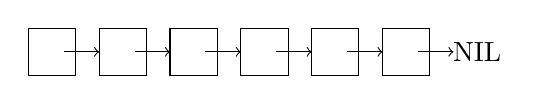
\begin{tikzpicture}[scale=3]
    \foreach \x in {-2, -1.7, ..., -0.4} {
      \draw (\x cm, 1cm) +(-0.1, -0.1) rectangle ++(0.1, 0.1);
      \draw[->] (\x cm, 1cm) +(0.05, 0) -- +(0.2, 0);
    }
    \draw (-0.2cm, 1cm) node {NIL};
    \end{tikzpicture}
  \caption{由节点组成的列表}
  \label{fig:list-example}
\end{figure}

每个节点要么链接到下一个节点上,要么指向NIL。通常使用复合数据结构\footnote{多数情况下,列表中元素有着共同的类型。有些环境(如Lisp)支持包含不同数据类型的列表。}定义列表,例如:

\lstset{frame=single}
\begin{lstlisting}[language=Bourbaki]
data List<A> {
    A key
    List<A> next
}
\end{lstlisting}

\index{列表!空} \index{列表!判空}

很多传统编程环境支持空引用NIL概念,存在两种不同的方法表示空列表:一种直接使用NIL(或null或$\nil$);另一种创建一个列表,但不填入任何元素,表示为$[\ ]$。在实现上,空引用不占用内存,但$[\ ]$则需要分配内存。

\subsection{分解}
\index{列表!头} \index{列表!尾} \index{列表!构造} \index{列表!cons}

给定一个非空列表$X$,我们定义两个函数\footnote{本书通常将函数调用$f(x)$记为$f\ x$,多元函数$f(x, y, ..., z)$记为$f\ x\ y\ ...\ z$。}来分别获取头部元素和子列表。它们通常被命名为\textit{first}\ $X$和\textit{rest}\ $X$,或者$head\ X$和$tail\ X$\footnote{在Lisp中,由于历史原因,它们被命名为\texttt{car}和\texttt{cdr}用以代表当时机器中的寄存器\cite{SICP}}。反之,我们可以从一个元素$x$和列表$xs$(可为空)构造出另一个列表,记为$x \cons xs$。这一构造过程也叫作cons。我们有如下关系:

\be
\begin{cases}
head\ (x \cons xs) & = x \\
tail\ (x \cons xs) & = xs
\end{cases}
\label{eq:list-head-tail}
\ee

我们也用$x_1$表示第一个元素,用$X'$表示剩余列表,例如$X = [x_1, x_2, x_3, ...]$,$X' = [x_2, x_3, ...]$。

\begin{Exercise}\label{ex:list-eq}
\Question{对于元素类型为$A$的列表,如果能够判断任何两个元素$x, y \in A$是否相等,定义一个算法来判断两个列表是否相等。}
\end{Exercise}

\begin{Answer}[ref={ex:list-eq}]
\Question{对于元素类型为$A$的列表,如果能够判断任何两个元素$x, y \in A$是否相等,定义一个算法来判断两个列表是否相等。
\begin{Haskell}
(==) :: [a] -> [a] -> Bool
[] == [] = True
(x:xs) == (y:ys) = x == y && (xs == ys)
xs == ys = False
\end{Haskell}
}
\end{Answer}

\subsection{列表的基本操作}
\index{列表!长度}
根据定义,我们可以递归地计算列表的长度:空列表的长度为0,而非空列表的长度是除去第一个元素的子列表长度加一。

\be
\begin{array}{rcl}
length\ [\ ] & = & 0 \\
length\ (x \cons xs) & = & 1 + length\ xs
\end{array}
\ee

因为遍历列表计算长度,其时间复杂度是$O(n)$,其中$n$是元素个数。在不和绝对值混淆的情况下,我们使用$|X|$来表示列表$X$的长度。为了避免反复计数,我们可以将长度存储在一个变量中,并在增加或删除元素时更新这一变量。下面是计算长度的迭代实现:

\begin{algorithmic}[1]
\Function{Length}{X}
  \State $n \gets 0$
  \While{$X \neq $ NIL}
    \State $n \gets n + 1$
    \State $X \gets $ \Call{Next}{$X$}
  \EndWhile
  \State \Return $n$
\EndFunction
\end{algorithmic}

\subsection{索引}
\index{列表!索引} \index{列表!get at}

数组支持以常数时间随机访问任意位置$i$的元素。但列表需要前进$i$步才能到达元素所在位置。

\be
getAt\ i\ (x \cons xs) = \begin{cases}
  i = 0: & x \\
  i \neq 0: & getAt\ (i - 1)\ xs \\
\end{cases}
\ee

我们故意没有处理空列表的情况。如果传入$[\ ]$,此时的行为是未定义的。$i$越界时的行为也是未定义的。若$i > |X|$,通过递归,最终转化为访问空列表的第$i - |X|$个位置的情况。另一方面,若$i < 0$,继续减一将使得它更偏离0,最终转化为访问空列表的某个负索引位置的情况。由于需要前进$i$步,索引算法的时间复杂度为$O(i)$。下面是对应的迭代实现:

\begin{algorithmic}[1]
\Function{Get-At}{$i, X$}
  \While{$i \neq 0$}
    \State $X \gets $ \Call{Next}{$X$}  \Comment{$X$ = NIL时出错}
    \State $i \gets i - 1$
  \EndWhile
  \State \Return \Call{First}{$X$}
\EndFunction
\end{algorithmic}

\begin{Exercise}\label{ex:list-get-at}
\Question{在\textproc{Get-At}($i, X$)的迭代实现中,$X$为空会怎样?$i$越界时会怎样?}
\end{Exercise}

\begin{Answer}[ref={ex:list-get-at}]
\Question{在\textproc{Get-At}($i, X$)的迭代实现中,$X$为空会怎样?$i$越界时会怎样?

此时的行为是未定义的。可以利用\texttt{Optional<T>}处理此种情况:
\begin{Bourbaki}
Optional<T> getAt(List<T> xs, Int i) {
    while i != 0 and xs != null {
        xs = xs.next
        i--
    }
    return if xs != null then Optional.of(xs.key) else Optional.Nothing
}
\end{Bourbaki}
}
\end{Answer}

\subsection{末尾元素}
\index{列表!末尾元素} \index{列表!init}

存在一对和first/rest对称的操作,称为last/init。对于非空列表$X = [x_1, x_2, ..., x_n]$,函数$last$返回末尾元素$x_n$,而$init$返回子列表$[x_1, x_2, ..., x_{n-1}]$。虽然这两对操作左右对称,但last/init需要遍历列表,因而是线性时间的。

\be
\begin{array}{cc}
  \begin{array}{rcl}
  last\ [x] & = & x \\
  last\ (x \cons xs) & = & last\ xs \\
  \end{array}
&
  \begin{array}{rcl}
  init\ [x] & = & [\ ] \\
  init\ (x:xs) & = & x : init\ xs \\
  \end{array}
\end{array}
\label{eq:list-last}
\ee

last/init都没有处理空列表的情况,当传入$[\ ]$时,行为是未定义的。下面是相应的迭代实现。

\begin{algorithmic}[1]
\Function{Last}{$X$}
  \State $x \gets $ NIL
  \While{$X \neq$ NIL}
    \State $x \gets $ \Call{First}{$X$}
    \State $X \gets $ \Call{Rest}{$X$}
  \EndWhile
  \State \Return $x$
\EndFunction
\Statex
\Function{Init}{$X$}
  \State $X' \gets $ NIL
  \While{\Call{Rest}{$X$} $\neq$ NIL} \Comment{$X$为NIL时出错}
    \State $X' \gets$ \textproc{Cons}(\Call{First}{$X$}, $X'$)
    \State $X \gets $ \Call{Rest}{$X$}
  \EndWhile
  \State \Return \Call{Reverse}{$X'$}
\EndFunction
\end{algorithmic}

\textproc{Init}通过\textproc{Cons}累积结果。这样产生的列表是逆序的,最后需要将结果再倒转过来(见第\ref{sec:reverse}节)。

\subsection{反向索引}
\index{列表!反向索引} \index{列表!rindex}

$last$是反向索引的一种特例。更一般的形式是获取列表中的倒数第$i$个元素。最直接的思路是遍历两次:第一次获取列表长度$n$,第二次获取第$n - i - 1$个元素:

\[
  lastAt\ i\ X = getAt\ (|X| - i - 1)\ L
\]

更好的解法是使用两个指针$p_1$和$p_2$,它们相距$i$步,即$rest^i(p_2) = p_1$,其中$rest^i(p_2)$表示重复执行函数$rest$共$i$次。也就是说,从$p_2$前进$i$步就可到达$p_1$。$p_2$一开始指向链表的头部,然后同时向前移动它们,直到$p_1$到达链表的尾部。此时指针$p_2$恰好指向倒数第$i$个元素。图\ref{fig:list-rindex}描述了这一方法。由于$p_1, p_2$框出一个窗口,这一方法也称作滑动窗口法。

\begin{figure}[htbp]
    \centering
    \subcaptionbox{$p_2$指向表头,距离$p_1$之后$i$步。}{\includegraphics[scale=0.8]{img/list-rindex}} \\
    \subcaptionbox{当$p_1$到达表尾时,$p_2$指向右数第$i$个。}{\includegraphics[scale=0.8]{img/list-rindex-2}}
    \caption{双指针滑动窗口}
    \label{fig:list-rindex}
\end{figure}

\begin{algorithmic}[1]
\Function{Last-At}{$i, X$}
  \State $p \gets X$
  \While{$i > 0$}
    \State $X \gets $ \Call{Rest}{$X$} \Comment{越界时出错}
    \State $i \gets i - 1$
  \EndWhile
  \While{\Call{Rest}{$X$} $\neq$ NIL}
    \State $X \gets$ \Call{Rest}{$X$}
    \State $p \gets$ \Call{Rest}{$p$}
  \EndWhile
  \State \Return \Call{First}{$p$}
\EndFunction
\end{algorithmic}

纯函数实现时不能直接更新指针,为此我们可以同时遍历$X = [x_1, x_2, ..., x_n]$和$Y = [x_i, x_{i+1}, ..., x_n]$,其中$Y$是除去前$i-1$个元素后的子列表。

\be
lastAt\ i\ X\ = slide\ X\ (drop\ i\ X)
\ee

其中:

\be
\begin{array}{rcl}
slide\ (x \cons xs)\ [y] & = & x \\
slide\ (x \cons xs)\ (y \cons ys) & = & slide\ xs\ ys \\
\end{array}
\ee

函数$drop\ m\ X$丢弃前$m$个元素:

\be
\begin{array}{rcl}
drop\ 0\ xs & = & xs \\
drop\ m\ [\ ] & = & [\ ] \\
drop\ m\ (x \cons xs) & = & drop\ (m - 1)\ xs \\
\end{array}
\ee

\begin{Exercise}\label{ex:list-init-last}
\Question{在\textproc{Init}中,可以用\textproc{Append}($X'$, \textproc{First}($X$))来替换\textproc{Cons}么?}
\Question{在\textproc{Last-At}中,如何处理空列表和越界的情况?}
\end{Exercise}

\begin{Answer}[ref={ex:list-init-last}]
\Question{在\textproc{Init}中,可以用\textproc{Append}($X'$, \textproc{First}($X$))来替换\textproc{Cons}么?
\textproc{Append}每次需要前进到末尾添加元素,这样使得复杂度从$O(n)$下降到$O(n^2)$,其中$n$是列表长度。
}
\Question{在\textproc{Last-At}中,如何处理空列表和越界的情况?
\begin{Bourbaki}
Optional<T> lastAt(List<T> xs, Int i) {
    List<T> p = xs
    while i != 0 and xs != null {
        xs = xs.next
        i--
    }
    if xs == null then return Optional.Nothing
    while xs.next != null {
        xs = xs.next
        p = p.next
    }
    return Optional.of(p.key)
}
\end{Bourbaki}
}
\end{Answer}

\subsection{更改}
\index{列表!更改}

更改操作包括添加、插入、更新、删除。某些函数式环境在实现时创建新列表,而原列表保持(persist)不变,并在适当的时候释放原始列表(\cite{okasaki-book},第2章)。

\index{列表!添加}
添加称为append,和cons对称,cons在表头增加,append在末尾增加。因此也被称作snoc(将cons反过来拼写)。由于要遍历到列表尾部,所以其复杂度为$O(n)$,其中$n$是列表的长度。为了避免反复遍历,我们可以将尾部位置存储下来,并随着列表变化进行更新。

\be
\begin{array}{rcl}
append\ [\ ]\  x & = & [x] \\
append\ (y \cons ys)\ x & = & y : append\ ys\ x \\
\end{array}
\ee

对应的迭代实现如下\footnote{参数的顺序也是对称的:$cons\ x\ xs$、$append\ xs\ x$。}:

\begin{algorithmic}[1]
\Function{Append}{$X, x$}
  \If{$X = $ NIL}
    \State \Return \Call{Cons}{$x$, NIL}
  \EndIf
  \State $H \gets X$ \Comment{保存表头}
  \While{\Call{Rest}{$X$} $\neq$ NIL}
    \State $X \gets$ \Call{Rest}{$X$}
  \EndWhile
  \State \Call{Rest}{$X$} $\gets$ \Call{Cons}{$x$, NIL}
  \State \Return $H$
\EndFunction
\end{algorithmic}

更新\textproc{Rest}的过程通常实现为对\texttt{next}引用的改写,如下面的例子代码:

\begin{lstlisting}[language=Bourbaki]
List<A> append(List<A> xs, A x) {
    if xs == null then return cons(x, null)
    var head = xs
    while xs.next != null {
        xs = xs.next
    }
    xs.next = cons(x, null)
    return head
}
\end{lstlisting}

\index{列表!修改}
和$getAt$类似,我们需要移动到列表中的指定位置以修改元素。

\be
\begin{array}{rcl}
setAt\ 0\ x\ (y \cons ys) & = & x : ys \\
setAt\ i\ x\ (y \cons ys) & = & y : setAt\ (i - 1)\ x\ ys \\
\end{array}
\ee

这一算法的时间复杂度为$O(i)$,其中$i$是要修改的位置。

\begin{Exercise}\label{ex:list-append}
\Question{在列表的定义中增加一个尾部变量tail,将添加算法优化为常数时间。}
\Question{何时应该更新tail变量?对性能有何影响?}
\Question{在$setAt$中,如何处理空列表和越界的情况?}
\end{Exercise}

\begin{Answer}[ref={ex:list-append}]
\Question{在列表的定义中增加一个尾部变量tail,将添加算法优化为常数时间。

我们需要两层定义,内层是基本的单向链表,外层是带有首尾变量的列表。
\begin{Bourbaki}
data List<A> {
    data Node<A> {
        A key
        Node<A> next
    }

    Node<A> head = null
    Node<A> tail = null
    Int length = 0
}

List<A> append(List<A> xs, A x) {
    List.Node<A> tl = xs.tail
    xs.tail = List.Node<A>(x, null)
    if tl == null {
        xs.head = xs.tail
    } else {
        tl.next = xs.tail
    }
    xs.length++
    return xs
}
\end{Bourbaki}
}
\Question{何时应该更新tail变量?对性能有何影响?

在尾部添加、删除时,向空列表加入节点时,从单一元素列表删除元素时,从中间位置分割列表时。除最后一个操作外,其它都是常数时间操作。从中间位置分割时$as = bs \doubleplus cs$,需要线性时间确定$bs$的尾部。
}
\Question{在$setAt$中,如何处理空列表和越界的情况?

$setAt\ 0\ x\ [\ ]$的意义等同于$x : [\ ]$。如果$|xs| = n$,可以认为$setAt\ n\ x\ xs$等价于$xs \doubleplus [x]$。其它空列表和越界情况可做异常处理。
}
\end{Answer}

\subsubsection{插入}
\index{列表!插入}

列表插入有两种不同的含义:(1)在指定位置插入一个元素,记为$insert\ i\ x\ X$,其实现和$setAt$类似;(2)在已序列表中插入一个元素,使得结果仍然是已序的。

\be
\begin{array}{rcl}
insert\ 0\ x\ ys & = & x : ys \\
insert\ i\ x\ (y \cons ys) & = & y : insert\ (i - 1)\ x\ ys \\
\end{array}
\ee

当$i$超过列表的长度时,我们可以将其视作添加,见本节习题。下面是相应的迭代实现:

\begin{algorithmic}[1]
\Function{Insert}{$i, x, X$}
  \If{$i = 0$}
    \State \Return \Call{Cons}{$x, X$}
  \EndIf
  \State $H \gets X$
  \State $p \gets X$
  \While{$i > 0$ and $X \neq$ NIL}
    \State $p \gets X$
    \State $X \gets $ \Call{Rest}{$X$}
    \State $i \gets i - 1$
  \EndWhile
  \State \Call{Rest}{$p$} $\gets$ \Call{Cons}{$x, X$}
  \State \Return $H$
\EndFunction
\end{algorithmic}

令列表$X = [x_1, x_2, ..., x_n]$已序,即对任何位置$1 \leq i \leq j \leq n$,有$x_i \leq x_j$。这里$\leq$的含义是抽象的,它可以代表任何有序的比较,包括$\geq$(降序)、集合的包含关系等。我们定义有序插入,使得列表保持有序。

\be
\begin{array}{rcl}
insert\ x\ [\ ] & = & [x] \\
insert\ x\ (y \cons ys) & = & \begin{cases}
  x \leq y : & x \cons y \cons ys \\
  \text{否则} : & y : insert\ x\ ys \\
  \end{cases}
\end{array}
\label{eq:list-ordered-insert}
\ee

由于要逐一比较元素,插入的时间复杂度为$O(n)$,其中$n$是长度。对应的迭代实现如下:

\begin{algorithmic}[1]
\Function{Insert}{$x, X$}
  \If{$X = $ NIL 或 $x <$ \Call{First}{$X$}}
    \State \Return \Call{Cons}{$x, X$}
  \EndIf
  \State $H \gets X$
  \While{\Call{Rest}{$X$} $\neq $ NIL 且 \textproc{First}(\Call{Rest}{$X$}) $< x$}
    \State $X \gets $ \Call{Rest}{$X$}
  \EndWhile
  \State \Call{Rest}{$X$} $\gets$ \textproc{Cons}($x$, \Call{Rest}{$X$})
  \State \Return $H$
\EndFunction
\end{algorithmic}

\label{sec:isort}
利用按序插入操作,我们可以实现插入排序:逐一将元素按序插入到一个空列表中。由于每次按序插入都是线性的,所以这一排序的复杂度为$O(n^2)$。

\be
\begin{array}{rcl}
sort\ [\ ] & = & [\ ] \\
sort\ (x \cons xs) & = & insert\ x\ (sort\ xs) \\
\end{array}
\ee

我们可以消除递归,实现一个迭代算法:逐一从列表中取出元素并按序插入到结果中:

\begin{algorithmic}[1]
\Function{Sort}{$X$}
  \State $S \gets$ NIL
  \While{$X \neq$ NIL}
    \State $S \gets$ \textproc{Insert}(\Call{First}{$X$}, $S$)
    \State $X \gets$ \Call{Rest}{$X$}
  \EndWhile
  \State \Return $S$
\EndFunction
\end{algorithmic}

在循环中的任何时刻,结果列表都是已序的。和递归实现相比,它们有一个本质不同:前者从右向左处理列表,而后者从左向右处理。我们稍后将在“尾递归”\ref{sec:tail-call}节中讲述如何消除这一差异。第3章详细介绍插入排序,包括性能分析和优化。

\begin{Exercise}\label{ex:list-insert}
\Question{当插入位置越界时,将其按照添加来处理。}
\Question{针对数组实现插入算法,插入位置$i$后的所有元素需要向后移动一个位置。}
\end{Exercise}

\begin{Answer}[ref = {ex:list-insert}]
\Question{当插入位置越界时,将其按照添加来处理。
\begin{Haskell}
insert n x [] = [x]
insert n x (y:ys) | n <= 0 = x : y : ys
                  | otherwise y : insert (n - 1) x ys
\end{Haskell}
}
\Question{针对数组实现插入算法,插入位置$i$后的所有元素需要向后移动一个位置。
\begin{Bourbaki}
[K] insert([K] xs, Int i, K x) {
    append(xs, x)
    for Int j = length(xs) - 1, j > i, j-- {
        swap(xs[j], xs[j-1])
    }
    return xs
}
\end{Bourbaki}
}
\end{Answer}

\subsubsection{删除}
\index{列表!删除}

和插入类似,删除也有两种含义:(1)在指定位置删除元素$delAt\ i\ X$;(2)查找某个值并删除$delete\ x\ X$。为了删除位置$i$的元素,我们首先前进$i$步到达目标位置,然后跳过一个元素,将剩余部分连接起来。

\be
\begin{array}{rcl}
delAt\ i\ [\ ] & = & [\ ] \\
delAt\ 0\ (x \cons xs) & = & xs \\
delAt\ i\ (x \cons xs) & = & x : delAt\ (i - 1)\ xs \\
\end{array}
\ee

由于需要前进$i$步执行删除,这一算法的时间复杂度为$O(i)$。下面是相应的迭代实现:

\begin{algorithmic}[1]
\Function{Del-At}{$i, X$}
  \State $S \gets$ \Call{Cons}{$\perp, X$} \Comment{辅助节点}
  \State $p \gets S$
  \While{$i > 0$ 且 $X \neq$ NIL}
    \State $i \gets i - 1$
    \State $p \gets X$
    \State $X \gets $ \Call{Rest}{$X$}
  \EndWhile
  \If{$X \neq$ NIL}
    \State \Call{Rest}{$p$} $\gets$ \Call{Rest}{$X$}
  \EndIf
  \State \Return \Call{Rest}{$S$}
\EndFunction
\end{algorithmic}

为了简化边界情况的处理,我们引入来一个辅助节点$S$,它包含一个特殊的值$\perp$,并指向$X$。使用$S$,我们可以安全地切除$X$中的任何节点,包括头节点。最后将$S$后继的部分作为结果返回,并丢弃$S$自身。“查找并删除”又可以进一步细分为两种情况:(1)仅找到第一个出现的元素并删除;(2)找到所有等于某值的元素全部删除。后者更加一般,见本节练习。

\be
\begin{array}{rcl}
delete\ x\ [\ ] & = & [\ ] \\
delete\ x\ (y \cons ys) & = & \begin{cases}
  x = y : & ys \\
  x \neq y : & y : delete\ x\  ys \\
  \end{cases} \\
\end{array}
\label{eq:list-delete}
\ee

由于需要遍历列表以查找待删除的元素,这一算法的复杂度为$O(n)$,其中$n$为长度。在迭代实现中,我们依然可以使用辅助节点来简化逻辑:

\begin{algorithmic}[1]
\Function{Delete}{$x, X$}
  \State $S \gets$ \Call{Cons}{$\perp, X$}
  \State $p \gets X$
  \While{$X \neq$ NIL 且 \Call{First}{$X$} $\neq x$}
    \State $p \gets X$
    \State $X \gets$ \Call{Rest}{$X$}
  \EndWhile
  \If{$X \neq$ NIL}
    \State \Call{Rest}{$p$} $\gets$ \Call{Rest}{$X$}
  \EndIf
  \State \Return \Call{Rest}{$S$}
\EndFunction
\end{algorithmic}

\begin{Exercise}\label{ex:list-delete}
\Question{设计算法将等于给定值的所有元素删除。}
\Question{设计数组的删除算法,被删除位置后的所有元素需要向前移动一个位置。}
\end{Exercise}

\begin{Answer}[ref = {ex:list-delete}]
\Question{设计算法将等于给定值的所有元素删除。
\begin{Haskell}
delAll x [] = []
delAll x (y:ys) | x == y = delAll x ys
                | otherwise = y : delAll x ys
\end{Haskell}
或使用叠加操作:
\begin{Haskell}
delAll x = foldr f [] where
  f y ys = if x == y then ys else y : ys
\end{Haskell}
}
\Question{设计数组的删除算法,被删除位置后的所有元素需要向前移动一个位置。
\begin{Bourbaki}
[K] delAt(Int i, [K] xs) {
    Int n = length(xs)
    if 0 <= i and i < n {
        while i < n - 1 {
            xs[i] = xs[i + 1]
            i++
        }
        popLast(xs)
    }
    return xs
}
\end{Bourbaki}
}
\end{Answer}

\subsubsection{连接}
\label{concat}
\index{列表!连接}

连接是添加操作的更一般形式,添加每次向列表尾部加入一个元素,而连接向列表尾部加入多个元素。但如果通过多次添加来实现,则整体操作的性能会下降为平方级别。令$|xs| = n$,$|ys| = m$,分别是两个列表的长度。每次添加都需要前进到尾部,总共添加$m$次。总时间复杂度为$O(n + (n + 1) + ... + (n + m)) = O(nm + m^2)$。

\[
\begin{array}{rcl}
xs \doubleplus [\ ] & = & xs \\
xs \doubleplus (y \cons ys) & = & append\ xs\ y \doubleplus ys \\
\end{array}
\]

而cons的速度很快(常数时间),我们可以前进到$xs$的尾部再链接到$ys$。

\be
\begin{array}{rcl}
[\ ] \doubleplus ys & = & ys \\
xs \doubleplus [\ ] & = & xs \\
(x \cons xs) \doubleplus ys & = & x : (xs \doubleplus ys) \\
\end{array}
\ee

改进实现的复杂度为$O(n)$。在命令式环境中,通过使用尾部引用,可以实现常数时间的连接操作(见本节习题)。

\begin{algorithmic}[1]
\Function{Concat}{$X, Y$}
  \If{$X = $ NIL}
    \State \Return $Y$
  \EndIf
  \If{$Y = $ NIL}
    \State \Return $X$
  \EndIf
  \State $H \gets X$
  \While{\Call{Rest}{$X$} $\neq$ NIL}
    \State $X \gets$ \Call{Rest}{$X$}
  \EndWhile
  \State \Call{Rest}{$X$} $\gets Y$
  \State \Return $H$
\EndFunction
\end{algorithmic}

\subsection{和与积}
\index{列表!和} \index{列表!积}
我们常常需要计算列表的和与积。它们有着共同的计算结构,在第\ref{sec:fold}节中,我们介绍如何对它们进行抽象。定义空列表的和为0、积为1。

\be
\begin{array}{cc}
  \begin{array}{rcl}
  sum\ [\ ] & = & 0 \\
  sum\ (x \cons xs) & = & x + sum\ xs \\
  \end{array}
  &
  \begin{array}{rcl}
  product\ [\ ] & = & 1 \\
  product (x \cons xs) & = & x \cdot product\ xs \\
  \end{array}
\end{array}
\ee

\index{尾递归} \index{尾调用} \index{尾递归调用}
\label{sec:tail-call}
两个算法都需要遍历整个列表,复杂度为$O(n)$,其中$n$为长度。求和、求积都从右向左计算。我们可以将其改成从左向右\textbf{累积计算}。求和时从0开始累加。求积时从1开始累乘。

\be
\begin{array}{cc}
  \begin{array}{rcl}
  sum'\ a\ [\ ] & = & a \\
  sum'\ a\ (x \cons xs) & = & sum\ (x + a)\ xs \\
  \end{array}
  &
  \begin{array}{rcl}
  prod'\ a\ [\ ] & = & a \\
  prod'\ a\ (x \cons xs) & = & prod'\ (x \cdot a)\ xs \\
  \end{array} \\
\end{array}
\ee

给定列表,我们以0为累积起始值调用$sum'$,以1为累积起始值调用$prod'$:

\be
sum\ xs = sum'\ 0\ xs
\quad \quad \quad
product\ xs = prod'\ 1\ xs
\ee

或使用柯里化形式:

\[
sum = sum'\ 0 \quad \quad \quad product = prod'\ 1
\]

\index{柯里化形式} \index{柯里化}
\textbf{柯里化}是肖芬格尔(Schönfinkel, 1889 - 1942)在1924年提出的。哈斯克尔·柯里在1958年后广泛使用\cite{slpj-book-1987}。考虑二元函数$f(x, y)$,如果只传入$x$,它就转换为一个关于$y$的一元函数:$g(y) = f(x, y)$,记为$g = f\ x$。推广到多元函数$f(x, y, ..., z)$,通过依次传入参数,可以转换为一系列函数:$f, f\ x, f\ x\ y, ...$。我们称这样的转换为柯里化。它可以把多元函数转化为一系列一元函数,即:$f(x, y, ..., z) = f(x)(y)...(z) = f\ x\ y\ ...\ z$。

采用累积法后,计算顺序变为从左向右,并且无需记录中间结果、状态用于递归。所有状态或作为参数(例如$a$)传入,或丢弃不用(例如已处理过的元素)。这样的递归可进一步转化为循环。我们称这样的函数为“尾递归”(或“尾调用”),称这种消除递归的优化为“尾递归优化”\cite{wiki-tail-call}。顾名思义,在这类函数中,递归发生在计算尾部。尾递归优化可以极大地提高性能,并避免由于递归过深造成的调用栈溢出。在第\ref{sec:isort}节关于插入排序的部分,其递归实现从右向左对元素排序。我们也可以将其转化为尾递归:

\be
\begin{array}{rcl}
sort'\ a\ [\ ] & = & a \\
sort'\ a\ (x \cons xs) & = & sort'\ (insert\ x\ a)\ xs \\
\end{array}
\ee

这样排序可以定义为传入$[\ ]$作为起始值的柯里化形式:$sort = sort'\ [\ ]$。作为尾递归的典型例子,我们考虑如何高效地计算幂$b^n$(\cite{SICP},1.16节。)。最直接的方法是从1开始重复乘以$b$共$n$次,这是一个$O(n)$时间的方法:

\begin{algorithmic}[1]
\Function{Pow}{$b, n$}
  \State $x \gets 1$
  \Loop{ $n$次}
    \State $x \gets x \cdot b$
  \EndLoop
  \State \Return $x$
\EndFunction
\end{algorithmic}

考虑计算$b^8$的过程,上述算法经过前两次迭代,可以得到$x = b^2$的结果。此时,我们无需用$x$乘以$b$得到$b^3$,可以直接再次乘以$b^2$,从而得到$b^4$。然后再次乘方,就可以得到$(b^4)^2 = b^8$。这样总共只要循环3次,而不是8次。若$n$恰好为2的整数次幂,即$n = 2^m$,其中$m$是非负整数,我们可以用下面的方法快速计算$b^n$:

\[
\begin{array}{rcl}
b^1 & = & b \\
b^n & = & (b^{\frac{n}{2}})^2 \\
\end{array}
\]

继续这一分治策略,我们可以将$n$推广到任意的非负整数:若$n = 0$,定义$b^0 = 1$;若$n$为偶数,将$n$减半,先计算$b^{\frac{n}{2}}$,然后再将结果平方;若$n$为奇数,因为$n-1$是偶数,可以先递归计算$b^{n-1}$,然后再将结果乘以$b$。

\be
\begin{array}{rcl}
b^0 & = & 1 \\
b^n & = & \begin{cases}
2 | n : & (b^{\frac{n}{2}})^2 \\
\text{否则} : & b \cdot b^{n-1} \\
\end{cases}
\end{array}
\ee

但是,第二条调用无法直接转换为尾递归。为此,我们可以先将底数平方,然后再将指数减半。

\be
\begin{array}{rcl}
b^0 & = & 1 \\
b^n & = & \begin{cases}
2 | n : & (b^2)^{\frac{n}{2}} \\
\text{否则} : & b \cdot b^{n-1} \\
\end{cases}
\end{array}
\ee

经过这一修改,就可以将算法转换为尾递归。我们通过等式$b^n = pow(b, n, 1)$计算幂。

\be
\begin{array}{rcl}
pow(b, 0, a) & = & a \\
pow(b, n, a) & = & \begin{cases}
  2 | n : & pow(b^2, \dfrac{n}{2}, a) \\
  \text{否则}: & pow(b, n - 1, ab) \\
\end{cases}
\end{array}
\ee

这一方法的性能为$O(\lg n)$。我们还可以继续改进,如果将$n$表示成二进制数$n = (a_ma_{m-1}...a_1a_0)_2$,如果$a_i = 1$,我们清楚地知道,需要计算$b^{2^i}$。这和二项式堆的情况很类似(第10章\autoref{sec:binomial-heap})。将所有二进制位为1的幂计算出,再累乘到一起就得到最后的结果。例如,当计算$b^{11}$时,11写成二进制为$11 = (1011)_2 = 2^3 + 2 +1$,因此$b^{11} = b^{2^3} \times b^2 \times b$。我们可以通过以下的步骤进行计算:

\begin{enumerate}
\item 计算$b^1$,得$b$;
\item 从这一结果进而得到$b^2$;
\item 将第2步的结果平方,从而得到$b^{2^2}$;
\item 将第3步的结果平方,得到$b^{2^3}$。
\end{enumerate}

最后,我们将第1、2、和第4步的结果乘到一起,得到$b^{11}$。综上,我们可以改进如下:

\be
\begin{array}{rcl}
pow(b, 0, a) & = & a \\
pow(b, n, a) & = & \begin{cases}
  2 | n : & pow(b^2, \dfrac{n}{2}, a) \\
  \text{否则}: & pow(b^2, \lfloor \dfrac{n}{2} \rfloor, ab) \\
  \end{cases}
\end{array}
\ee

这一算法本质上每次将$n$向右移动一个二进制位(通过将$n$除以2)。若最低位(LSB: Least Significant Bit)为0,$n$为偶数。我们将底数平方,继续递归,无需改变累积结果$a$。这对应上面例子的第3步;若LSB为1,$n$为奇数。除了将底数平方,还要将$b$乘到累积结果$a$上;当$n$为0时,我们已处理完$n$中的所有位,最终结果就是累积值$a$。在任何时候,更新的底数$b'$,移位后的指数$n'$,和累积结果$a$总满足不变条件$b^n = a (b')^{n'}$。此前的算法当$n$为奇数时,仅仅将其减一转化为偶数进行处理;这一改进每次都将$n$减半。若$n$的二进制表示中有$m$位,这一算法只计算$m$轮。当然它的复杂度仍然为$O(\lg n)$。我们将这一算法的命令式实现作为练习。

回到求和、求积问题。在迭代实现中,我们一边遍历,一边应用加法或乘法累积结果:

\begin{algorithmic}[1]
\Function{Sum}{$X$}
  \State $s \gets 0$
  \While{$X \neq$ NIL}
    \State $s \gets s +$ \Call{First}{$X$}
    \State $X \gets$ \Call{Rest}{$X$}
  \EndWhile
  \State \Return $s$
\EndFunction
\Statex
\Function{Product}{$X$}
  \State $p \gets 1$
  \While{$X \neq$ NIL}
    \State $p \gets p\ \cdot$ \Call{First}{$X$}
    \State $X \gets$ \Call{Rest}{$X$}
  \EndWhile
  \State \Return $p$
\EndFunction
\end{algorithmic}

利用求积算法,我们可以将阶乘实现为递推方式:$n! = product\ [1..n]$。

\subsection{最大值和最小值}
\index{列表!最大值} \index{列表!最小值}

如果非空有限列表中的元素可进行比较,则存在最大、最小值。$\max/\min$的计算结构相同:若列表中只有一个元素$[x_1]$,结果为$x_1$;否则,递归地在子列表中寻找最大、最小值,并和表头元素比较得到最终结果。

\be
\resizebox{\linewidth}{!}{\ensuremath{
\begin{array}{cc}
  \begin{array}{rcl}
  \min\ [x] & = & x \\
  \min\ (x \cons xs) & = & \begin{cases}
    x < \min\ xs : & x \\
    \text{否则}: & \min\ xs \\
  \end{cases}
  \end{array}
&
  \begin{array}{rcl}
  \max\ [x] & = & x \\
  \max\ (x \cons xs) & = & \begin{cases}
    x > \max\ xs : & x \\
    \text{否则}: & \max\ xs \\
  \end{cases}
  \end{array}
\end{array}
}}
\ee

这两个实现都从右向左处理,我们可以将其变为尾递归。并且这样还具备了“在线”处理能力,即任何时候,累积结果都是已处理部分中的最大、最小值。以$min$为例:

\be
\begin{array}{rcl}
\min'\ a\ [\ ] & = & a \\
\min'\ a\ (x \cons xs) & = & \begin{cases}
  x < a : & \min'\ x\ xs \\
  \text{否则} : & \min'\ a\ xs \\
  \end{cases}
\end{array}
\ee

与$sum'/prod'$不同,我们不能向$\min'/\max'$传入一个常数作为起始值,除非使用$\pm \infty$(柯里化形式):

\[
  \textstyle \min = \min'\ \infty \quad \quad \quad \max = \max'\ -\infty
\]

考虑到最大、最小值仅对非空列表有定义,可以将表头元素传入作为累积起始值:

\be
  \textstyle
  \min\ (x \cons xs) = \min'\ x\ xs
  \quad \quad \quad
  \max\ (x \cons xs) = \max'\ x\ xs
\ee

尾递归的最大、最小值算法可以进一步转化为迭代实现。我们略过\textproc{Max}以\textproc{Min}为例:

\begin{algorithmic}[1]
\Function{Min}{$X$}
  \State $m \gets$ \Call{First}{$X$}
  \State $X \gets$ \Call{Rest}{$X$}
  \While{$X \neq$ NIL}
    \If{\Call{First}{$X$} $< m$ }
      \State $m \gets$ \Call{First}{$X$}
    \EndIf
    \State $X \gets$ \Call{Rest}{$X$}
  \EndWhile
  \State \Return $m$
\EndFunction
\end{algorithmic}

还有一种尾递归实现,可以复用表头元素作为累积器。递归时,由于列表中至少有两个元素,我们每次拿出前两个比较,丢弃一个,然后继续处理剩余的元素。以$\min$为例,$\max$的实现与此对称。

\be
\begin{array}{rcl}
\min\ [x] & = & x \\
\min\ (x_1 \cons x_2 \cons xs) & = & \begin{cases}
  x_1 < x_2 : & \min\ (x_1 \cons xs) \\
  \text{否则}: & \min\ (x_2 \cons xs) \\
  \end{cases}
\end{array}
\ee

\begin{Exercise}\label{ex:list-tail-recursive}
\Question{使用尾递归实现$length$}
\Question{使用尾递归实现插入排序。}
\Question{使用$n$的二进制形式,实现幂$b^n$的快速计算,使得复杂度为$O(\lg n)$}
\end{Exercise}

\begin{Answer}[ref = {ex:list-tail-recursive}]
\Question{使用尾递归实现$length$
\begin{Haskell}
length  = len 0 where
  len n [] = n
  len n (x:xs) = len (n + 1) xs
\end{Haskell}
}
\Question{使用$n$的二进制形式,实现幂$b^n$的快速计算,使得复杂度为$O(\lg n)$

我们并不要求$b$一定是整数,甚至是实数。$b$可以是任何定义了单位$e$(例如1)和二元运算(例如乘法)的集合。数学上我们称这样的集合为幺半群(Monoid)。
\begin{Bourbaki}
Monoid pow(Monoid b, Int n) {
    Monoid a = Monoid.e
    while n != 0 {
        if n & 1 == 1 then a = a * b
        b = b * b
        n = n >> 1
    return a
}
\end{Bourbaki}
}
\end{Answer}

\section{变换}
\index{列表!变换}

从代数角度看,有两种不同的变换:一种保持列表结构,仅仅改变元素;另一种改变列表结构,变换结果和原列表不再同构。特别地,我们称保持列表结构的变换为\textbf{逐一映射}。

\subsection{逐一映射}
\index{列表!逐一映射}
我们通过一些例子来认识映射。第一个例子将一列数字映射为代表它们的字符串,如把[3, 1, 2, 4, 5]转换为[``three'', ``one'', ``two'', ``four'', ``five'']。

\be
\begin{array}{rcl}
toStr\ [\ ] & = & [\ ] \\
toStr\ (x \cons xs) & = & (str\ x) : toStr\ xs \\
\end{array}
\label{eq:tostr}
\ee

第二个例子是关于单词统计的。考虑一个字典,包含若干单词,并以它们的首字母分组,例如:

\begin{Verbatim}[fontsize=\footnotesize]
[[a, an, another, ... ],
 [bat, bath, bool, bus, ...],
 ...,
 [zero, zoo, ...]]
\end{Verbatim}

接下来我们处理一段文章,例如《王子复仇记》,统计各单词在其中的出现次数:

\begin{Verbatim}[fontsize=\footnotesize]
[[(a, 1041), (an, 432), (another, 802), ... ],
 [(bat, 5), (bath, 34), (bool, 11), (bus, 0), ...],
 ...,
 [(zero 12), (zoo, 0), ...]]
\end{Verbatim}

现在我们要找出,对应每个首字母,哪个单词被使用的次数最多?输出结果是一个单词列表,表中每个单词都是在各自首字母组中出现最多的一个,形如:\texttt{[a, but, can, ...]}。我们需要设计一个程序,将一组单词/次数对的列表转换成一个单词列表。首先定义一个函数,接受一个单词/次数对列表,找出次数最多的单词。我们无需排序,只需要实现某种特殊的$maxBy\ cmp\ xs$,其中$cmp$是抽象的比较函数。

\be
\begin{array}{rcl}
maxBy\ cmp\ [x] & = & x \\
maxBy\ cmp\ (x_1 \cons x_2 \cons xs) & = & \begin{cases}
  cmp\ x_1\ x_2 : & maxBy\ cmp\ (x_2 \cons xs) \\
  \text{否则} : & maxBy\ cmp\ (x_1 \cons xs) \\
  \end{cases}
\end{array}
\ee

对于一对值(也叫做数偶)$p = (a, b)$,定义辅助函数:

\be
\begin{cases}
fst\ (a, b) = & a \\
snd\ (a, b) = & b \\
\end{cases}
\ee

定义单词/次数对的比较函数:

\be
less\ p_1\ p_2 = snd\ p_1 < snd\ p_2
\ee

将$less$传入$maxBy$就可选出出现次数最多的单词(柯里化):$\max'' = maxBy\ less$。最后,调用$\max''$处理单词统计列表:

\be
\begin{array}{rcl}
solve\ [\ ] & = & [\ ] \\
solve\ (x \cons xs) & = & (fst\ (\max''\ x)) : solve\ xs \\
\end{array}
\label{eq:solve}
\ee

\index{列表!映射}
尽管解决的问题不同,$solve$和$toStr$反映出同样的计算结构。我们将这样的结构抽象为\textbf{逐一映射}。

\be
\begin{array}{rcl}
map\ f\ [\ ] & = & [\ ] \\
map\ f\ (x \cons xs) & = & (f\ x) : map\ f\ xs \\
\end{array}
\ee

$map$接受一个函数$f$作为参数,然后将其应用到列表中的每个元素上。我们称将其它函数作为计算对象的函数为“高阶函数”。如果$f$的类型为$A \to B$,即把类型$A$的元素映射为类型$B$的元素,则$map$的类型为:

\be
map :: (A \to B) \to [A] \to [B]
\ee

读作:$map$接受一个类型为$A \to B$的函数,然后将一个类型为$[A]$的列表变换为另一个类型为$[B]$的列表。上面的两个例子可以使用映射定义如下(柯里化):

\[
\textstyle
toStr = map\ str \quad \quad \quad
solve = map\ (fst \circ \max'')
\]

其中$f \circ g$表示函数组合,它首先应用函数$g$,然后再应用函数$f$,即$(f \circ g)\ x = f(g(x))$。读作$f$作用于$g$之后。我们也可以从集合论的角度来定义映射。函数$y = f(x)$定义了一个从集合$X$中的元素$x$到集合$Y$中的元素$y$的映射:

\be
Y = \{ f(x) | x \in X \}
\ee

\index{列表!ZF表达式} \index{列表!列表解析}
这种形式定义出的集合称为“策梅罗——弗兰克尔”集合抽象(简称ZF表达式)\cite{algo-fp}。不同之处在于,我们定义的是从列表$X$到列表$Y$的映射$Y = [f(x) | x \gets X]$,而不是集合的映射。其中可以含有重复元素。列表的ZF表达式被称作“列表解析”,它是一个强大的工具。作为例子,我们思考如何实现一个排列算法。我们从全排列\cite{algo-fp}\cite{erlang}出发,定义更一般的排列函数$perm\ X\ r$,列举从长度为$n$的列表$X$中选出$r$个元素的全部排列。一共有$P_n^r = \dfrac{n!}{(n-r)!}$种不同的排列。

\be
\resizebox{\linewidth}{!}{\ensuremath{
perm\ X\ r = \begin{cases}
  |X| < r\ \text{或}\ r = 0: & [[\ ]] \\
  \text{否则}: & [ x\cons ys \ |\ x \gets X, ys \gets perm\ (delete\ x\ X)\ (r - 1)] \\
  \end{cases}
}}
\ee

如果选出0个元素排列,或列表中元素的个数小于$r$,排列结果为空列表的列表[[\ ]];否则,我们逐一取出列表中每个元素$x$,递归地从剩余的$n-1$个元素中选择$r-1$个元素排列,然后再将$x$置于每个排列的前面。

为了简化映射的迭代实现,下面的算法中使用了一个辅助节点。

\begin{algorithmic}[1]
\Function{Map}{$f, X$}
  \State $X' \gets$ \Call{Cons}{$\perp$, NIL} \Comment{辅助节点}
  \State $p \gets X'$
  \While{$X \neq$ NIL}
    \State $x \gets$ \Call{First}{$X$}
    \State $X \gets$ \Call{Rest}{$X$}
    \State \Call{Rest}{$p$} $\gets$ \Call{Cons}{$f(x)$, NIL}
    \State $p \gets$ \Call{Rest}{$p$}
  \EndWhile
  \State \Return \Call{Rest}{$X'$} \Comment{丢弃辅助节点}
\EndFunction
\end{algorithmic}

\index{列表!for each}
某些情况下我们只希望逐一处理表中的每个元素,而无需构造新的列表。例如打印一个列表中的每个元素:

\begin{algorithmic}[1]
\Function{Print}{$X$}
  \While{$X \neq$ NIL}
    \State print \Call{First}{$X$}
    \State $X \gets$ \Call{Rest}{$X$}
  \EndWhile
\EndFunction
\end{algorithmic}

通常,我们在遍历时传入一个过程$P$,然后遍历列表,将$P$应用到每个元素上。

\begin{algorithmic}[1]
\Function{For-Each}{$P, X$}
  \While{$X \neq$ NIL}
    \State \textproc{P}(\Call{First}{$X$})
    \State $X \gets$ \Call{Rest}{$X$}
  \EndWhile
\EndFunction
\end{algorithmic}

作为例子,我们思考一下“$n$盏灯”趣题\cite{poj-drunk-jailer}:屋子里有$n$盏灯,都是熄灭的。我们执行下面的过程$n$次。

\begin{enumerate}
\item 将所有的灯都打开;
\item 扳动第2、4、6……盏灯的开关。如果灯是亮的,则熄灭;如果是灭的,则点亮;
\item 每三个灯,扳动一次开关。第3、6、9……位置上的灯的明暗状态切换;
\item ……
\end{enumerate}

最后一轮的时候,只有最后一盏灯(第$n$盏)的开关被扳动。问最终有几盏灯是亮的?考虑穷举法。把$n$盏灯表示为一列0、1数字(0灭、1亮)。开始时都是灭的[0, 0, ..., 0]。将灯编号为1到$n$,然后映射成一个关于($i$, 亮/灭)的列表:

\[
lights = map\ (i \mapsto (i, 0))\ [1, 2, ..., n]
\]

这一映射将每个编号都对应到0,结果列表由$n$个数偶组成:$L$ = [(1, 0), (2, 0), ..., ($n$, 0)]。操作$L$共$n$次。在第$i$次中,逐一检查每对值$(j, x)$,若$i | j$(即$j \bmod i = 0$)就翻转亮/灭。考虑$1 - 0 = 1$且$1 - 1 = 0$,可将亮灭状态$x$切换为$1 - x$。

\be
switch\ i\ (j, x)) = \begin{cases}
  j \bmod i = 0 : & (j, 1 - x) \\
  \text{否则}: & (j, x) \\
  \end{cases}
\ee

第$i$轮操作实现为$map\ (switch\ i)\ L$。这里使用了$switch$的柯里化形式。接下来定义函数$op$,执行映射$n$次$op\ [1, 2, ..., n]\ L$。

\be
\begin{array}{rcl}
op\ [\ ]\ L & = & L \\
op\ (i \cons is)\ L & = & op\ is\ (map\ (switch\ i)\ L) \\
\end{array}
\ee

最后,将数偶中第二个元素累加起来就得到答案。

\be
solve\ n = sum\ (map\ snd\ (op\ [1, 2, ..., n]\ L))
\ee

下面的Haskell例子程序实现了穷举法。

\begin{Haskell}
solve = sum . (map snd) . proc  where
    lights = map (\i -> (i, 0)) [1..n]
    proc n = operate [1..n] lights
    operate [] xs = xs
    operate (i:is) xs = operate is (map (switch i) xs)
    switch i (j, x) = if j `mod` i == 0 then (j, 1 - x) else (j, x)
\end{Haskell}

我们列出灯的数目为1、2、……、100盏时的答案(人为添加了换行):

\begin{Verbatim}[fontsize=\footnotesize]
[1,1,1,
 2,2,2,2,2,
 3,3,3,3,3,3,3,
 4,4,4,4,4,4,4,4,4,
 5,5,5,5,5,5,5,5,5,5,5,
 6,6,6,6,6,6,6,6,6,6,6,6,6,
 7,7,7,7,7,7,7,7,7,7,7,7,7,7,7,
 8,8,8,8,8,8,8,8,8,8,8,8,8,8,8,8,8,
 9,9,9,9,9,9,9,9,9,9,9,9,9,9,9,9,9,9,9,10]
\end{Verbatim}

这一结果很有规律:3盏灯以内时,最后有1盏灯亮;4盏到8盏灯时,最后有2盏灯亮;9盏到15盏灯时,最后有3盏灯亮;……看起来灯的数目为$i^2$到$(i+1)^2-1$盏时,最后有$i$盏灯亮。我们可以证明这一结论:

\begin{proof}
将$n$盏灯编号为1到$n$,考虑最后仍然亮的那些灯。由于初始时,所有灯都是灭的,我们可以确定,被扳动奇数次开关的灯最后是亮的。对于编号为$i$的灯,若$i$可以被$j$整除(表示为$j | i$),则在第$j$轮,它的开关被扳动一次。所以当灯的编号含有奇数个因子时,最后的状态是亮的。为了找出最后亮的灯,我们需要找出所有含有奇数个因子的数。对于任意自然数$n$,记$S$为$n$的所有因子的集合。$S$初始化为$\varnothing$,若$p$为$n$的一个因子,则必然存在一个正整数$q$,使得$n = p q$。也就是说$q$也是$n$的因子。因此当且仅当$p \neq q$时,我们向集合$S$中添加两个不同的因子,这样$|S|$将总是偶数。除非$p = q$,此时$n$必定是完全平方数。这时只能向集合$S$中增加一个因子,从而导致奇数个因子。
\end{proof}

我们可以寻找$n$以内的完全平方数来解决这一趣题。

\be
solve(n) = \lfloor \sqrt{n} \rfloor
\ee

下面的Haskell例子程序输出1、2、……、100盏灯时的结果:

\begin{Haskell}
map (floor . sqrt) [1..100]
\end{Haskell}

映射是一个抽象概念,它不仅局限于列表,也可以扩展到许多复杂的代数结构。下一章我们会介绍如何对树结构进行映射。只要我们能够遍历一个结构,并且有空结构的定义,就可以使用映射的概念。

\subsection{反转}
\index{列表!反转} \label{sec:reverse}

如何用最小的空间反转一个单向链表是一道经典题目,需要仔细操作节点的引用。有一个简单的策略:(1)先写出一个纯递归解;(2)转换为尾递归;(3)将尾递归转换为命令式操作。纯递归解很直观:

\[
\begin{array}{rcl}
reverse [\ ] & = & [\ ] \\
reverse (x \cons xs) & = & append\ (reverse\ xs)\ x \\
\end{array}
\]

接下来进行尾递归优化。使用一个累积器来记录反转结果,并传入空列表来启动:$reverse = reverse'\ [\ ]$。

\be
\begin{array}{rcl}
reverse'\ a\ [\ ] & = & a \\
reverse'\ a\ (x \cons xs) & = & reverse'\ (x \cons a)\ xs \\
\end{array}
\ee

不同于在尾部添加,cons(:)是常数时间操作。我们不断从列表的头部逐一取出元素,将其置于累积结果的前面。这相当于将全部元素压入一个堆栈,然后再依次弹出。整体上是线性时间的。由于尾递归无需记录上下文环境,我们可以将其优化为循环迭代:

\begin{algorithmic}[1]
\Function{Reverse}{$X$}
  \State $A \gets$ NIL
  \While{$X \neq$ NIL}
    \State $A \gets $ \textproc{Cons}(\Call{First}{$X$}, $A$)
    \State $X \gets$ \Call{Rest}{$X$}
  \EndWhile
  \State \Return $A$
\EndFunction
\end{algorithmic}

但是,这一算法生成了一个新的反转列表,而不是在原列表上直接修改。我们接下来要通过重用$X$将其改为就地修改的形式。如下面的例子程序:

\begin{lstlisting}[language=Bourbaki]
List<T> reverse(List<T> xs) {
    List<T> p, ys = null
    while xs != null {
        p = xs
        xs = xs.next
        p.next = ys
        ys = p
    }
    return ys
}
\end{lstlisting}

\begin{Exercise}\label{ex:list-transform}
\Question{使用尾递归求$[(k, v)]$列表中$v$值最大的元素。}
\end{Exercise}

\begin{Answer}[ref = {ex:list-transform}]
\Question{使用尾递归求$[(k, v)]$列表中$v$值最大的元素。
\begin{Haskell}
maxValue ((k, v):kvs) = maxV v kvs where
  maxV m [] = m
  maxV m ((_, v):kvs) = maxV (max m v) kvs
\end{Haskell}
}
\end{Answer}

\section{子列表}
\index{列表!提取子列表} \index{列表!截取} \index{列表!丢弃} \index{列表!分割}

数组可以快速地分割为连续的切片,而列表分割则需要遍历,因而这类操作都是线性时间的。$take$从列表中取出前$n$个元素,相当于获取从第1到第$n$个元素的的子列表:$sublist\ 1\ n\ X$。$drop$从列表中丢弃前$n$个元素,等价于从右侧获取子列表$sublist\ (n+1)\ |X|\ X$。它和$take$对称\footnote{有些语言内置了这两个操作,例如Python中:\texttt{xs[:m]}和\texttt{xs[m:]}分别相当于$take/drop$。}:

\be
\resizebox{\linewidth}{!}{\ensuremath{
\begin{array}{cc}
  \begin{array}{rcl}
  take\ 0\ xs & = & [\ ] \\
  take\ n\ [\ ] & = & [\ ] \\
  take\ n\ (x \cons xs) & = & x : take\ (n - 1)\ xs \\
  \end{array}
&
  \begin{array}{rcl}
  drop\ 0\ xs & = & xs \\
  drop\ n\ [\ ] & = & [\ ] \\
  drop\ n\ (x \cons xs) & = & drop\ (n - 1)\ xs \\
  \end{array}
\end{array}
}}
\ee

这一算法是这样处理越界情况的:如果$n > |X|$或$n$为负数,最终转化为$X$为空的边界情况。我们把对应的迭代实现留作本节习题。使用取出和丢弃操作,可以在列表的任何位置获取指定长度的子列表。

\be
sublist\ from\ cnt\ X = take\ cnt\ (drop\ (from - 1)\ X)
\ee

另外一种形式,是传入左侧和右侧的边界:

\be
slice\ from\ to\ X = drop\ (from - 1)\ (take\ to\ X)
\ee

\index{List!split at}
闭区间$[from, to]$包括两端。我们也可以在指定位置把列表分割开:

\be
splitAt\ i\ X = (take\ i\ X, drop\ i\ X)
\label{eq:split-at}
\ee

\index{列表!条件截取} \index{列表!条件丢弃}
\textit{take/drop}指定截取或丢弃的个数。我们可以对其扩展,只要某种条件成立,就不断取出或者丢弃元素,称为\textit{takeWhile/dropWhile}。它们逐一检查元素是否满足给定条件$p$,如果不满足,则停止检查剩余的部分,这和后面介绍的过滤算法有所不同。

\be
\resizebox{\linewidth}{!}{\ensuremath{
\begin{array}{cc}
  \begin{array}{rcl}
  \textit{takeWhile}\ p\ [\ ] & = & [\ ] \\
  \textit{takeWhile}\ p\ (x \cons xs) & = & \begin{cases}
    (p\ x) : & x : \textit{takeWhile}\ p\ xs \\
    \text{否则}: & [\ ] \\
    \end{cases}
  \end{array}
&
  \begin{array}{rcl}
  \textit{dropWhile}\ p\ [\ ] & = & [\ ] \\
  \textit{dropWhile}\ p\ (x \cons xs) & = & \begin{cases}
    (p\ x) : & \textit{dropWhile}\ p\ xs \\
    \text{否则}: & x \cons xs \\
    \end{cases}
  \end{array}
\end{array}
}}
\ee

\subsection{切分和分组}
\index{列表!切分} \index{列表!break} \index{列表!span}

切分和分组操作将列表中的元素重新安排成若干子列表。通常一边遍历一边进行这种分类安排,使得时间复杂度为线性。切分可以被认为是一种特殊的\textit{split},我们不是在指定的位置将列表分开,而是检查每个元素是否满足某一条件,根据条件找出最长前缀。切分结果是一对子列表,一个是最长前缀,另一个包含剩余的部分。切分有两种类型:一种是满足条件的最长子列表;另一种是\textbf{不}满足条件的最长子列表。前者称为$span$,后者称为$break$。

\be
\begin{array}{rcl}
span\ p\ [\ ] & = & ([\ ], [\ ]) \\
span\ p\ (x \cons xs) & = & \begin{cases}
  (p\ x) : & (x \cons as, bs)\ \text{其中}\ (as, bs) = span\ p\ xs \\
  \text{否则}: & ([\ ], x \cons xs) \\
  \end{cases}
\end{array}
\label{eq:span}
\ee

只需要把条件取逻辑非,就可以实现$break\ p = span\ (\lnot p)$。$span$和$break$都寻找最长\textbf{前缀}。一旦条件打破就立即停下,忽略剩余部分。下面是\textproc{Span}的迭代实现:

%% \begin{algorithmic}[1]
%% \Function{Span}{$p, X$}
%%   \State $A \gets $ NIL
%%   \While{$X \neq$ NIL and $p$(\Call{First}{$X$})}
%%     \State $A \gets $ \textproc{Cons}(\Call{First}{$X$}, $A$)
%%     \State $X \gets $ \Call{Rest}{$X$}
%%   \EndWhile
%%   \State \Return $(A, X)$
%% \EndFunction
%% \end{algorithmic}

%% 这一实现创建了新列表用以存放最长前缀,也可以复用原列表的空间,转换为就地修改。

\begin{algorithmic}[1]
\Function{Span}{$p, X$}
  \State $A \gets X$
  \State $tail \gets$ NIL
  \While{$X \neq$ NIL 且 $p$(\Call{First}{$X$})}
    \State $tail \gets X$
    \State $X \gets $ \Call{Rest}{$X$}
  \EndWhile
  \If{$tail =$ NIL}
    \State \Return (NIL, $X$)
  \EndIf
  \State \Call{Rest}{$tail$} $\gets$ NIL
  \State \Return $(A, X)$
\EndFunction
\end{algorithmic}

\index{列表!分组}
$span$和$break$将列表切分为两部分,分组将列表中的元素分成若干子列表。例如将字符串分割为若干子串,每个包含连续相同字符:

\[
\textit{group}\ \text{``Mississippi''} = [\text{``M'', ``i'', ``ss'', ``i'', ``ss'',``i'', ``pp'', ``i''}]
\]

再例如,给出一列数字:$X$ = [15, 9, 0, 12, 11, 7, 10, 5, 6, 13, 1, 4, 8, 3, 14, 2],把它分成若干组,每组中的元素按降序排列:

\[
\textit{group}\ X = [[15, 9, 0], [12, 11, 7], [10, 5], [6], [13, 1], [4], [8, 3], [14, 2]]
\]

这两个例子都具有实用价值。字符串分组后,可构造基数树用于快速文本搜索(第6章)。有序子列表可实现自然归并排序(第13章)。我们把分组条件抽象成某种关系$\sim$。它用于判断两个相邻元素$x$、$y$是否“等价”:$x \sim y$。我们遍历列表,每次比较两个元素。如果等价,就把它们置于一组;否则把$x$、$y$分置于两组中。

\be
\resizebox{\linewidth}{!}{\ensuremath{
\begin{array}{rcl}
group\ \sim\ [\ ] & = & [[\ ]] \\
group\ \sim\ [x] & = & [[x]] \\
group\ \sim\ (x \cons y \cons xs) & = & \begin{cases}
  x \sim y : & (x \cons ys) \cons yss, \text{其中}: (ys \cons yss) = group\ \sim\ (y \cons xs) \\
  \text{否则}: & [x] \cons ys \cons yss \\
\end{cases}
\end{array}
}}
\ee

这一算法的时间复杂度为$O(n)$,其中$n$是长度。也可以用迭代的方式实现这一算法。若$X$不为空,我们将分组结果初始化为$[[x_1]]$。然后从第二个元素开始遍历列表,若相邻的两个元素“等价”,我们就将遍历到的元素放入最后一组,否则就新创建一个组。

\begin{algorithmic}[1]
\Function{Group}{$\sim, X$}
  \If{$X = $ NIL}
    \State \Return [[\ ]]
  \EndIf
  \State $x \gets$ \Call{First}{$X$}
  \State $X \gets$ \Call{Rest}{$X$}
  \State $g \gets [x]$
  \State $G \gets [g]$
  \While{$X \neq$ NIL}
    \State $y \gets$ \Call{First}{$X$}
    \If{$x \sim y$}
      \State $g \gets $ \Call{Append}{$g, y$}
    \Else
      \State $g \gets [y]$
      \State $G \gets$ \Call{Append}{$G, g$}
    \EndIf
    \State $x \gets y$
    \State $X \gets$ \Call{Next}{$X$}
  \EndWhile
  \State \Return $G$
\EndFunction
\end{algorithmic}

如果添加\textproc{Append}没有尾部引用优化,这一实现的时间复杂度会退化为$O(n^2)$。如果不关心顺序,可以将\textproc{Append}改为\textproc{Cons}。使用分组函数,本节开头的两个例子可实现为:$\textit{group}\ (=)\ \text{``Mississippi''}$和$\textit{group}\ (\geq)\ X$。也可以使用$span$来实现分组。传入一个条件,$span$将列表分割成两部分:其中之一是满足条件的最长子列表。我们对剩余部分不断执行\textit{span}处理完所有元素。但是传入\textit{span}的条件函数是一元函数,而分组条件要求是二元函数。可以用柯里化来解决这一差异:将第一个元素传入二元判断函数并固定。

\be
\resizebox{\linewidth}{!}{\ensuremath{
\begin{array}{rcl}
group\ \sim\ [\ ] & = & [[\ ]] \\
group\ \sim\ (x \cons xs) & = & (x \cons as) : group\ \sim\ bs, \text{其中}: (as, bs) = span\ (y \mapsto x \sim y)\ xs \\
\end{array}
}}
\ee

\index{等价关系}
虽然这个新函数可以将文本中的相同字母分组,但却不能正确地把数字按降序分组:$\textit{group}\ (\geq)\ X$ = [[15,9,0,12,11,7,10,5,6,13,1,4,8,3,14,2]]。第一个元素是15,它被置于$\geq$的左侧进行比较。15是列表中的最大元素,因此\textit{span}把所有元素都置于$as$中,而$bs$为空。这并不是错误,而是正确的行为。因为分组被设计为将“等价”的元素放到一起。严格说来,等价关系($\sim$)条件必须满足三个性质:自反性、传递性、对称性。

\begin{enumerate}
\item \textbf{自反性}:$x \sim x$;
\item \textbf{传递性}:$x \sim y, y \sim z \Rightarrow x \sim z$;
\item \textbf{对称性}:$x \sim y \Leftrightarrow y \sim x$。
\end{enumerate}

对``Mississippi''分组时,使用等号($=$),上述三个条件都满足,产生了正确结果。但将柯里化的大于等于号($\geq$)作为等价关系时,违反了自反性和对称性,因而无法按预期分组。用\textit{span}实现的第二个分组算法,将含义限制为更严格的等价关系,而第一个分组算法则无此限制。它仅检查任何两个相邻元素是否满足条件,这比等价条件要弱。

\begin{Exercise}\label{ex:list-take-drop}
\Question{修改$take/drop$,当$n$是负数时$take$返回$[\ ]$,$drop$返回全部列表。}
\Question{实现就地修改的take和drop算法。}
\Question{将$sublist$和$slice$改写为柯里化形式,无需$X$作为参数。}
\Question{考虑下面$span$的实现:
\[
\begin{array}{rcl}
span\ p\ [\ ] & = & ([\ ], [\ ]) \\
span\ p\ (x \cons xs) & = & \begin{cases}
  (p\ x) : & (x:as, bs), \text{其中}: (as, bs) = span(p, xs) \\
  \text{否则}: & (as, x:bs) \\
\end{cases}
\end{array}
\]
它和我们本节给出的实现有何不同?}
\end{Exercise}

\begin{Answer}[ref = {ex:list-take-drop}]
\Question{修改$take/drop$,当$n$是负数时$take$返回$[\ ]$,$drop$返回全部列表。
\begin{Haskell}
safeTake n [] = []
safeTake n (x:xs) | n <= 0 = []
                  | otherwise = x : safeTake (n - 1) xs

safeDrop n [] = []
safeDrop n (x:xs) | n <= 0 = x:xs
                  | otherwise = drop (n - 1) xs
\end{Haskell}
}
\Question{实现就地修改的take和drop算法。

需要在数组尾部加入、删除元素。在头部或中间则需要shift操作。令数组$xs$长度为$n$,$take(m, xs)$可以通过连续进行$n - m$次尾部删除实现。为了实现$drop(m, xs)$,从$xs[m]$起,把每个元素$xs[i]$向前移动到$xs[i - m]$。最后从尾部删除$m$个元素。
\begin{Bourbaki}
[K] take(Int m, [K] xs) {
    Int d = length(xs) - m
    while d > 0 and xs != [] {
        pop(xs)
        d--
    }
    return xs
}

[K] drop(Int m, xs) {
    if m <= 0 then return xs
    for Int i = m to length(xs) { xs[i - n] = xs[i] }
    while m > 0 and xs != [] {
        pop(xs)
        m--
    }
    return xs
}
\end{Bourbaki}
}
\Question{将$sublist$和$slice$改写为柯里化形式,无需$X$作为参数。
\begin{Haskell}
sublist from cnt = take cnt . drop (from - 1)

slice from to = drop (from - 1) . take to
\end{Haskell}
}
\Question{考虑下面$span$的实现:
\[
\begin{array}{rcl}
span\ p\ [\ ] & = & ([\ ], [\ ]) \\
span\ p\ (x \cons xs) & = & \begin{cases}
  (p\ x) : & (x:as, bs), \text{其中}: (as, bs) = span(p, xs) \\
  \text{否则}: & (as, x:bs) \\
\end{cases}
\end{array}
\]
它和我们本节给出的实现有何不同?

这一实现把列表$xs$分成了两部分:满足$p$的所有元素和不满足$p$的所有元素:$as = [p(a), a \gets xs]$和$bs = [not\ p(b), b \gets xs]$。$as$不一定是满足$p$的最长前缀,而是满足$p$的最长子序列。
}
\end{Answer}


\section{叠加}
\label{sec:fold}
\index{叠加} \index{列表!foldr} \index{列表!右侧叠加}
几乎所有的列表算法都有着共同的结构。这不是一个巧合。这种共性本质上来自列表的递归性质。我们可以将列表算法抽象到更高层次的概念:叠加\footnote{也叫作reduce}。它本质上是所有列表计算的初始代数\cite{unplugged}。比较$sum$、$product$、$sort$,它们都有共同的结构:列表为空时的结果,求和时为0、求积时为1、排序时为$[\ ]$;对表头元素和递归结果进行二元运算,求和时是相加、求积时是相乘、排序时是按序插入。我们将空列表时的结果抽象为\textbf{初始值}$z$(抽象的零),二元运算抽象为$\oplus$。定义如下结构:

\be
\begin{array}{rcl}
h\ \oplus\ z\ [\ ] & = & z \\
h\ \oplus\ z\ (x \cons xs) & = & x \oplus (h\ \oplus\ z\ xs) \\
\end{array}
\ee

输入列表$X = [x_1, x_2, ..., x_n]$,计算过程展开如下:

\[
\begin{array}{rl}
   & h\ \oplus\ z\ [x_1, x_2, ..., x_n] \\
= & x_1 \oplus (h\ \oplus\ z\ [x_2, x_3, ..., x_n]) \\
= & x_1 \oplus (x_2 \oplus (h\ \oplus\ z\ [x_3, ..., x_n])) \\
  & ... \\
= & x_1 \oplus (x_2 \oplus (... (x_n \oplus (h\ \oplus\ z\ [\ ]))...)) \\
= & x_1 \oplus (x_2 \oplus (... (x_n \oplus z)...))
\end{array}
\]

这些括弧是必须的,它限制计算顺序从最右侧开始($x_n \oplus z$),不断向左侧进行直到$x_1$。这和图\ref{fig:fold-fan}描述的折扇相似。折扇由竹子和纸制成。多根扇骨在末端被轴穿在一起。把展开的扇形逐渐折叠,最终收起成一根。

\begin{figure}[htbp]
  \centering
  
\includegraphics[scale=0.4]{img/fold-fan}
  \caption{折扇}
  \label{fig:fold-fan}
\end{figure}

这些扇骨组成了一个列表。收起扇子的二元操作是将一根扇骨叠在已收起的部分之上。最初的收起部分为空。收起的过程从一端开始,不断应用二元操作,直到所有的扇骨都叠在一起。求和与求积算法和收起折扇的过程是相同的。

\[
\resizebox{\linewidth}{!}{\ensuremath{
\begin{array}{cc}
  \begin{array}{rl}
  sum\ [1, 2, 3, 4, 5 ] & = 1 + (2 + (3 + (4 + 5))) \\
           & = 1 + (2 + (3 + 9)) \\
           & = 1 + (2 + 12) \\
           & = 1 + 14 \\
           & = 15
  \end{array}
&
  \begin{array}{rl}
  product\ [1, 2, 3, 4, 5 ] & = 1 \times (2 \times (3 \times (4 \times 5))) \\
           & = 1 \times (2 \times (3 \times 20)) \\
           & = 1 \times (2 \times 60) \\
           & = 1 \times 120 \\
           & = 120
  \end{array}
\end{array}
}}
\]

我们称这一过程为\textbf{叠加}。特别地,由于计算从右侧一端开始,我们将其记为$foldr$:

\be
\begin{array}{rcl}
foldr\ f\ z\ [\ ] & = & z \\
foldr\ f\ z\ (x \cons xs) & = & f\ x\ (foldr\ f\ z\ xs) \\
\end{array}
\ee

使用$foldr$,求和与求积可以定义如下:

\be
\begin{array}{rl}
\sum_{i=1}^{n} x_i & = x_1 + (x_2 + (x_3 + ... + (x_{n-1} + x_{n}))...) \\
             & = foldr\ (+)\ 0\ [x_1, x_2, ..., x_n]
\end{array}
\ee

\be
\begin{array}{rl}
\prod_{i=1}^{n} x_i & = x_1 \times (x_2 \times (x_3 \times ... + (x_{n-1} \times x_{n}))...) \\
         & = foldr\ (\times)\ 1\ [x_1, x_2, ..., x_n]
\end{array}
\ee

或者写成柯里化形式:$sum = foldr\ (+)\ 0$和$product = foldr\ (\times)\ 1$。插入排序算法可定义为:$sort = foldr\ insert\ [\ ]$。

\index{列表!foldl} \index{列表!左侧叠加}
我们可以把$foldr$转换为尾递归,计算是从左向右进行的。我们将其记为$foldl$:

\be
\begin{array}{rcl}
foldl\ f\ z\ [\ ] & = & z \\
foldl\ f\ z\ (x \cons xs) & = & foldl\ f\ (f\ z x)\ xs \\
\end{array}
\ee

以$sum$为例,可以看到计算是自左向右展开的:

\[
\begin{array}{rl}
 & foldl\ (+)\ 0\ [1, 2, 3, 4, 5] \\
= & foldl\ (+)\ (0 + 1)\ [2, 3, 4, 5 ] \\
= & foldl\ (+)\ (0 + 1 + 2)\ [3, 4, 5] \\
= & foldl\ (+)\ (0 + 1 + 2 + 3)\ [4, 5] \\
= & foldl\ (+)\ (0 + 1 + 2 + 3 + 4)\ [5] \\
= & foldl\ (+)\ (0 + 1 + 2 + 3 + 4 + 5)\ [\ ] \\
= & 0 + 1 + 2 + 3 + 4 + 5 \\
\end{array}
\]

每一步都推迟了$f\ z\ x$的计算,这是惰性求值时的行为。否则每次调用的求值序列为$[1, 3, 6, 10, 15]$。一般来说,$foldl$可以展开为下面的形式(中缀记法):

%% \be
%% foldl\ f\ z\ [x_1, x_2, ..., x_n] = f\ (f\ ...\ (f\ (f\ z\ x_1)\ x_2)\ ... )\ x_n
%% \ee

\be
foldl\ (\oplus)\ z\ [x_1, x_2, ..., x_n] = z \oplus x_1 \oplus x_2 \oplus ... \oplus x_n
\ee

\index{reduce}
$foldl$是尾递归的,可以将其实现为循环。通常称作\textproc{Reduce}。

\begin{algorithmic}[1]
\Function{Reduce}{$f, z, X$}
  \While{$X \neq$ NIL}
    \State $z \gets f(z, $ \Call{First}{$X$} $)$
    \State $X \gets$ \Call{Rest}{$X$}
  \EndWhile
  \State \Return $z$
\EndFunction
\end{algorithmic}

$foldr$和$foldl$各自有适合的应用场景,它们并不总能互换。例如,某些容器只支持从一端添加元素(如栈)。我们要定义一个$\textit{fromList}$函数,从一个列表构建出容器(柯里化):

\[
\textit{fromList} = foldr\ add\ \nil
\]

其中$\nil$是空容器。单向链表本身就是这样一种容器。在头部添加元素的性能要远高于在尾部添加。如果希望复制列表并保持顺序,$foldr$就是一个自然的选择,而$foldl$则产生逆序的列表。在迭代实现时为了解决逆序问题,我们可以先反转列表,再执行reduce操作:

\begin{algorithmic}[1]
\Function{Reduce-Right}{$f, z, X$}
  \State \Return \textproc{Reduce}($f, z$, \Call{Reverse}{$X$})
\EndFunction
\end{algorithmic}

有人认为应优先使用$foldl$,因为它是尾递归的,同时满足函数式和命令式场景,并且还是在线算法。但在处理无穷列表(用流和惰性求值实现)时,就只能用$foldr$。下面的例子程序将一个无穷列表中的每个元素都置于一个单独的列表中,并返回前10个:

\[
\begin{array}{l}
take\ 10\ (foldr\ (x\ xs \mapsto [x] \cons xs)\ [\ ]\ [1, 2, ...]) \\
\Rightarrow [[1], [2], [3], [4], [5], [6], [7], [8], [9], [10]]
\end{array}
\]

这里不能使用$foldl$,否则计算永远不会完成。当左右没有区别时,我们用统一的符号$fold$。本书也使用符号$fold_l$和$fold_r$来强调叠加本身而非方向。尽管本章内容是关于列表的,但是叠加概念是抽象的。它可以应用到其它代数结构。我们可以对树(\cite{unplugged}2.6节)、队列和更复杂的结构进行叠加。只要它满足下面这两个条件:(1)定义了空(例如空树);(2)可分解的递归结构(例如一棵树可分解为子树和元素)。人们进一步将这些概念抽象为可叠加、幺半群、可遍历等等。

作为例子,我们来看如何用$fold$和$map$来解决$n$盏灯趣题。在穷举法中,我们创建了一个列表,每个元素是一对值$(i, s)$,包含灯的序号$i$和明暗状态$s$。每轮中操作中,如果灯的序号$i$能被轮数$j$整除,就翻转灯的状态。这一过程可以用$fold$定义:

\[
foldr\ step\ [(1, 0), (2, 0), ..., (n, 0)]\ [1, 2, ..., n]
\]

初始时所有灯都是灭的。要折叠的列表是从1到$n$的轮数。函数$step$接受两个参数:轮数$i$和“灯序号/状态”列表$step\ i\ L\ = map\ (switch\ i)\ L$。$foldr$的结果是最终的序号/明暗状态列表。接下来用$map$从每对值中提取出状态,再用$sum$求出有几盏灯是点亮的:

\be
sum\ (map\ snd\ (foldr\ step\ [(1, 0), (2, 0), ..., (n, 0)]\ [1, 2, ..., n]))
\ee

\index{列表!串联}
如果用“$\doubleplus$”(第\ref{concat}节)在一组列表上折叠,相当于把它们串联成一个列表。这和数字累加是类似的:

\be
concat = fold_r\ (\doubleplus)\ [\ ]
\ee

例如:$concat\ [[1], [2, 3, 4], [5, 6, 7, 8, 9]] \Rightarrow [1, 2, 3, 4, 5, 6, 7, 8, 9]$。

\begin{Exercise}\label{ex:list-fold}
\Question{为了用$foldr$定义插入排序,我们将插入函数设计成$insert\ x\ X$,这样排序可以表示为:$sort = foldr\ insert\ [\ ]$。$foldr$的类型为:
\[
foldr :: (A \to B \to B) \to B \to [A] \to B
\]
其中第一个参数$f$的类型是:$A \to B \to B$,初始值$z$的类型为$B$。它对元素类型为$A$的列表进行叠加,最终结果的类型为$B$。如何用$foldl$定义插入排序?$foldl$的类型是什么?}
\Question{$concat$的时间复杂度是什么?设计一个线性时间的$concat$算法。}
\Question{使用$foldr$来定义$map$。}
\end{Exercise}

\begin{Answer}[ref = {ex:list-fold}]
\Question{为了用$foldr$定义插入排序,我们将插入函数设计成$insert\ x\ X$,这样排序可以表示为:$sort = foldr\ insert\ [\ ]$。$foldr$的类型为:
\[
foldr :: (A \to B \to B) \to B \to [A] \to B
\]
其中第一个参数$f$的类型是:$A \to B \to B$,初始值$z$的类型为$B$。它对元素类型为$A$的列表进行叠加,最终结果的类型为$B$。如何用$foldl$定义插入排序?$foldl$的类型是什么?

\vspace{3mm}

$foldl$的类型为:$foldl :: (B \to A \to B) \to B \to [A] \to B$。使用$foldl$,我们需要对调参数的位置定义插入排序:
\[
sort = foldl\ (xs\ x \mapsto insert\ x\ xs)\ [\ ]
\]

或者定义一个“对调”函数:
\be
flip\ f\ x\ y = f\ y\ x
\ee

这样插入排序可定义为:$sort = foldl\ (flip\ insert)\ [\ ]$
}
\Question{$concat$的时间复杂度是什么?设计一个线性时间的$concat$算法。

使用$foldl$和$foldr$定义$concat$的结果大相径庭。$as \doubleplus bs$的复杂度是$O(m)$,其中$m = |as|$,使用$foldl$实现$xs_1 \doubleplus xs_2 \doubleplus ... \doubleplus xs_n$时,$as$的长度越来越长,复杂度为:$O(m_1 + (m_1 + m_2) + ... + \sum_1^{n-1} m_i)$。使用$foldr$实现$xs_1 \doubleplus (xs_2 \doubleplus (... \doubleplus xs_n)...)$时,$as$的长度不会越来越长,而是每个$xs_i$的长度,其复杂度为$O(m_{n-1} + ... + m_2 + m_1)$是线性时间的。我们可以展开定义一算法:

\begin{Haskell}
concat [] = []
concat ([]:xss) = concat xss
concat ((x:xs):xss) = x : concat (xs:xss)
\end{Haskell}
}
\Question{使用$foldr$来定义$map$。
\be
map\ f = foldr\ (x\ xs \mapsto (f\ x) \cons xs)\ [\ ]
\ee
}
\end{Answer}

\section{查找和过滤}

\index{列表!存在检查} \index{列表!属于}
查找和过滤都是抽象概念,不仅限于列表,也可用于更广泛的对象。对于列表,通常需要遍历以找到结果。最基本的操作是判断元素$x$是否属于列表$X$?我们可以遍历列表将每个元素和$x$进行对比。

\be
\begin{array}{rcl}
a \in [\ ] & = & False \\
a \in (b:bs) & = & \begin{cases}
  b = a : & True \\
  b \neq a : & a \in bs \\
  \end{cases}
\end{array}
\ee

这一操作也称作$elem$,复杂度为$O(n)$,其中$n$是列表长度。即使列表有序,仍然无法直接优化到$O(\lg n)$。这是因为列表不支持常数时间的随机访问,无法使用二分查找(见第3章)。

\index{列表!查询(lookup)}
接下来扩展$elem$操作。在$n$盏灯趣题中,我们使用了“键/值”对列表$[(k, v)]$。每对元素包含键、值,称作“关联列表”。我们希望通过某个键查询到其对应的值。

\be
\begin{array}{rcl}
lookup\ x\ [\ ] & = & \textit{Nothing} \\
lookup\ x\ ((k, v) \cons kvs) & = & \begin{cases}
  k = x: & Just\ (k, v) \\
  k \neq x: & lookup\ x\ kvs \\
  \end{cases}
\end{array}
\ee

和$elem$不同,我们不仅想知道$x$存在与否,还希望找到对应的值。由于键$x$并不一定存在,我们引入了“可能”代数类型$\mathbf{Maybe}\ A$,它有两种不同的值:类型$A$的某个值$a$或是空。分别记为$Just\ a$或\textit{Nothing}。这是一种解决空引用的方法\footnote{类似于某些编程环境的\texttt{Optional<A>}。}(\cite{unplugged}4.2.2节)。

\index{列表!查找(find)} \index{列表!过滤}
进一步扩展$lookup$到一般情况。不再比较是否等于某个值,而是查找满足某一条件的元素:

\be
\begin{array}{rcl}
find\ p\ [\ ] & = & \textit{Nothing} \\
find\ p\ (x \cons xs) & = & \begin{cases}
  (p\ x) : & Just\ x \\
  \text{否则}: & find\ p\ xs \\
  \end{cases}
\end{array}
\ee

尽管可能有多个元素满足条件,$find$只返回第一个。我们可以把它扩展为查找全部满足条件的元素,这一过程通常称作过滤,如图\ref{fig:filter}所示。其定义为(ZF表达式):$filter\ p\ X = [x | x \gets X, p\ x]$。

\begin{figure}[htbp]
   \centering
      \begin{tikzpicture}[scale=0.8]
      \draw (2, 0) rectangle (4, 1) node (filter) [pos=.5] {filter $p$};
      \draw (0, .5) node (in) {输入}
            (6, .5) node (out) {输出};
      \draw[thick, ->] (in) edge (filter)
                       (filter) edge (out);
      \end{tikzpicture} \\
   \caption{输入:$[x_1, x_2, ..., x_n]$,输出:$[x_1', x_2', ..., x_m']$。满足:$\forall x_i' \Rightarrow p(x_i')$.}
   \label{fig:filter}
\end{figure}

和$find$不同,如果没有任何元素满足条件,$filter$返回空列表。它逐一扫描列表,检查每个元素:

\be
\begin{array}{rcl}
filter\ p\ [\ ] & = & [\ ] \\
filter\ p\ (x \cons xs) & = & \begin{cases}
  (p\ x): & x : filter\ p\ xs \\
  \text{否则}: & filter\ p\ xs \\
  \end{cases}
\end{array}
\ee

这一算法从右向左构造结果。在迭代实现中,如果用\textproc{Append}来构造结果,性能会下降到$O(n^2)$。如果用\textproc{Cons}替代,则结果是逆序的。我们可以再执行一次线性时间的反转(见练习)。

\begin{algorithmic}[1]
\Function{Filter}{$p, X$}
  \State $X' \gets$ NIL
  \While{$X \neq$ NIL}
    \If{$p$(\Call{First}{$X$})}
      \State $X' \gets$ \textproc{Append}($X'$, \Call{First}{$X$}) \Comment{线性时间}
    \EndIf
    \State $L \gets$ \Call{Rest}{$X$}
  \EndWhile
\EndFunction
\end{algorithmic}

从右向左进行计算的过程可以用$foldr$来定义。设计函数$f$检查每个元素,如果符合条件就添加到结果中:$f\ p\ x\ as\ = \textbf{if}\ p\ x\ \textbf{then}\ x \cons as\ \textbf{else}\ as$。定义过滤为(柯里化):

\be
filter\ p = foldr\ (x\ as \mapsto f\ p\ x\ as)\ [\ ]
\ee

可以进一步简化为(称作$\eta$变换\cite{slpj-book-1987}):

\be
filter\ p = foldr\ (f\ p)\ [\ ]
\ee

过滤是一个通用的概念。不仅限于列表,可以对任何可遍历的结构应用某个判定条件,过滤出感兴趣的部分。

\index{列表!匹配} \index{列表!前缀} \index{列表!后缀} \index{列表!中缀}

匹配一般是指在一个结构中寻找某一模式。即使限定为列表和字符串,匹配仍是一个广泛、深入的内容(第14章)。我们仅考虑检查列表$as$是否出现在列表$bs$中的问题。这里有两个特例:判断$as$是否是$bs$的前缀、后缀。$span$寻找符合某个条件的最长前缀。使用类似的方法逐一比较$as$、$bs$中每个元素。若$as$是$bs$的前缀,记为:$as \subseteq bs$。

\be
\begin{array}{rcl}
[\ ] \subseteq bs & = & True \\
(a \cons as) \subseteq [\ ] & = & False \\
(a \cons as) \subseteq (b \cons bs) & = & \begin{cases}
  a \neq b: & False \\
  a = b: & as \subseteq bs \\
  \end{cases}
\end{array}
\ee

由于扫描列表,前缀检查是线性时间的。但我们不能用同样的方法来检查后缀:对齐尾部,然后从右向左比较。这一点与数组不同。为了实现线性时间的后缀检查,可以反转两个列表,转换为前缀检查:

\be
A \supseteq B = reverse(A) \subseteq reverse(B)
\ee

使用$\subseteq$,可以解决子列表问题(中缀检查)。定义空列表是任何列表的中缀,遍历列表$B$不断进行前缀检查:

\be
\begin{array}{rcl}
\textit{infix}?\ (a \cons as)\ [\ ] & = & False \\
\textit{infix}?\ A\ B & = & \begin{cases}
  A \subseteq B: & True \\
  \text{否则}: & \textit{infix}?\ A\ B' \\
  \end{cases}
\end{array}
\ee

下面是对应的迭代实现:

\begin{algorithmic}[1]
\Function{Is-Infix}{$A, B$}
  \If{$A = $ NIL}
    \State \Return TRUE
  \EndIf
  \State $n \gets |A|$
  \While{$B \neq$ NIL 且 $n \leq |B|$}
    \If{$A \subseteq B$}
      \State \Return TRUE
    \EndIf
    \State $B \gets$ \Call{Rest}{$B$}
  \EndWhile
  \State \Return FALSE
\EndFunction
\end{algorithmic}

由于前缀检测需要线性时间,并且在遍历时被不断调用,这一算法的复杂度为$O(nm)$,其中$n$和$m$分别是两个列表的长度。对称地,我们可以枚举出$B$的所有后缀,然后检查$A$是否是某个后缀的前缀:

\be
\textit{infix}?\ A\ B = \exists S \in \textit{suffixes}\ B, A \subseteq S
\ee

下面的Haskell例子程序使用列表解析实现了这一方法:

\begin{Haskell}
isInfixOf a b = (not . null) [s | s <- tails b, a `isPrefixOf` s]
\end{Haskell}

其中\texttt{isPrefixOf}进行前缀检查。\texttt{tails}枚举一个列表的所有后缀(本节练习)。

\begin{Exercise}\label{ex:list-query}
%% \Question{实现迭代的查询算法。}
\Question{使用$reverse$实现线性时间的过滤算法。}
\Question{实现迭代的前缀检查算法。}
\Question{给定一个列表,枚举出它的所有后缀。}
\end{Exercise}

\begin{Answer}[ref = {ex:list-query}]
%% \Question{实现迭代的查询算法。
%% \begin{Bourbaki}
%% Optional<K> lookup(K x, [(K, v)] assoc) {
%%     for k, v in assoc {
%%         if x == k then return Optional.of(v)
%%     }
%%     return Optional.Nothing
%% }
%% \end{Bourbaki}
%% }
\Question{使用$reverse$实现线性时间的过滤算法。
\begin{Bourbaki}
List<K> filterL((K -> Bool) p, List<K> xs) {
    List<K> ys = null
    while xs != null {
        if p(xs.key) then ys = cons(xs.key, ys)
        xs = xs.next
    }
    return reverse(ys)
}

List<K> reverse(List<K> xs) {
    List<K> ys = null
    while xs != null {
        ys = cons(xs.key, ys)
        xs = xs.next
    }
    return ys
}
\end{Bourbaki}
}
%% \Question{实现迭代的前缀检查算法。}
\Question{给定一个列表,枚举出它的所有后缀。

有多种方法。从列表$xs$开始,不断$drop$并记录下结果直到空串。
\[
[xs, drop\ xs, drop\ (drop\ xs), ..., [\ ]]
\]
也可以利用pattern matching不断去掉头部,实现drop的效果:
\begin{Haskell}
tails [] = [[]]
tails xs@(_:ys) =  xs : tails ys
\end{Haskell}

我们还可以利用右侧叠加从$[[\ ]]$开始,不断从右侧加入元素构造后缀:
\begin{Haskell}
tails = foldr f [[]] where
  f x xss@(xs:_) = (x:xs) : xss
\end{Haskell}
}
\end{Answer}

\section{关联和分解}
\index{列表!zip} \index{列表!unzip}

关联列表是一种简易映射(字典),用以处理少量数据。它比树、堆简单,但性能是线性的。在$n$盏灯趣题中,我们用逐一映射创建关联列表:$map\ (i \mapsto (i, 0))\ [1, 2, ..., n]$。为了“关联”两个列表,定义$zip$函数:

\be
\begin{array}{rcl}
zip\ as\ [\ ] & = & [\ ] \\
zip\ [\ ]\ bs & = & [\ ] \\
zip\ (a \cons as)\ (b \cons bs) & = & (a, b) : zip\ as\ bs \\
\end{array}
\ee

这一定义可处理长度不同的列表。关联结果的长度将和较短的一个相同。我们甚至可以关联无穷列表(利用惰性求值),例如\footnote{或$zip\ (repeat\ 0)\ [1..n]$,其中$repeat\ x = x : repeat\ x$}:$zip\ [0, 0, ...]\ [1, 2, ..., n]$。给定单词列表,我们可以给每个单词顺序编号为:$zip$ [1, 2, ...]\ [a, an, another, ...]。$zip$从右向左构建结果。我们可以用$foldr$定义它。复杂度为$O(m)$,其中$m$是较短列表的长度。在迭代实现时,如果使用\textproc{Append},其性能会下降为平方时间。可以使用\textproc{Cons}再反转结果。但无法处理无穷列表。在命令式环境中,可以复用$A$来存储结果(视为一种映射:将一列元素映射为一列元素对)。

\begin{algorithmic}[1]
\Function{Zip}{$A, B$}
  \State $C \gets$ NIL
  \While{$A \neq$ NIL 且 $B \neq$ NIL}
    \State $C \gets $ \textproc{Append}(C, (\Call{First}{$A$}, \Call{First}{$B$})) \Comment{线性时间}
    \State $A \gets$ \Call{Rest}{$A$}
    \State $B \gets$ \Call{Rest}{$B$}
  \EndWhile
  \State \Return $C$
\EndFunction
\end{algorithmic}

进一步扩展$zip$关联多个列表,有些编程环境提供了\texttt{zip}、\texttt{zip3}、\texttt{zip4}……。有时我们要应用某种组合函数,而不仅是构建元素对。例如,给定水果单价的列表:苹果、橙子、香蕉……单价为$[1.00, 0.80, 10.05, ...]$(元);顾客购买数量为:$[3, 1, 0, ...]$,表示购买了3个苹果,1个橙子、0个香蕉。下面的程序计算应付金额:

\[
\begin{array}{rcl}
pays\ us\ [\ ] & = & [\ ] \\
pays\ [\ ]\ qs & = & [\ ] \\
pays\ (u \cons us)\ (q \cons qs) & = & uq : pays\ us\ qs \\
\end{array}
\]

除了用乘法代替cons,其计算结构和$zip$相同。我们将组合函数抽象为$f$并传给$zip$定义出一般关联操作:

\be
\begin{array}{rcl}
zipWith\ f\ as\ [\ ] & = & [\ ] \\
zipWith\ f\ [\ ]\ bs & = & [\ ] \\
zipWith\ f\ (a \cons as)\ (b \cons bs) & = & (f\ a\ b) : zipWith\ f\ as\ bs \\
\end{array}
\ee

利用$zipWith$可以定义内积(点积)\cite{wiki-dot-product}:$A \cdot B = sum\ (zipWith\ (\cdot)\ A\ B)$。$zipWith$结合惰性求值还可以定义无穷斐波那契数列:

\be
F = 0 : 1 : zipWith\ (+)\ F\ F'
\ee

它的含义是$F$是无穷的斐波那契数列,第一个元素是0,第二个元素是1。$F'$是去掉头部元素的无穷斐波那契数列。从第三个元素起,每个斐波那契数,都是$F$和$F'$中对应元素的和。下面的例子程序列出了前15个斐波那契数:

\begin{Haskell}
fib = 0 : 1 : zipWith (+) fib (tail fib)

take 15 fib
[0,1,1,2,3,5,8,13,21,34,55,89,144,233,377]
\end{Haskell}

$zip$的逆运算是$unzip$,将关联列表分解成两个列表。可以使用$foldr$定义分解(柯里化):

\be
unzip = foldr\ ((a, b)\ (as, bs) \mapsto (a \cons as, b \cons bs))\ ([\ ], [\ ])
\ee

对于买水果的例子,若单价信息以关联列表的形式给出:$U$ = [(apple, 1.00), (orange, 0.80), (banana, 10.05), ...],购买数量也是关联列表:$Q$ = [(apple, 3), (orange, 1), (banana, 0), ...]。计算总金额时,从两个关联列表中分解出单价和数量,然后计算其内积:

\be
pay = sum\ (zipWith\ (\cdot)\ snd(unzip\ U)\ snd(unzip\ Q))
\ee

$zip$和$unzip$的概念是抽象的。我们可以扩展$zip$以关联两棵树,节点中的数据是元素对,分别来自两棵树中。抽象的$zip$和$unzip$还可以用于跟踪复杂结构的遍历路径,从而模拟命令式环境中的父节点引用(\cite{learn-haskell}的最后一章)。

列表是构建复杂数据结构和算法的基础,对于函数式编程尤为重要。我们介绍了构建、分解、更改、变换列表的基本算法;介绍了如何在列表中搜索、过滤、进行计算。尽管大多数编程环境都提供了工具来支持列表,我们不应仅把它们看作黑盒子。Rabhi和Lapalme\cite{algo-fp}介绍了关于列表的许多函数式算法。Haskell标准库提供了关于基础算法的详细文档。伯德\cite{fp-pearls}给出了很多与叠加相关的例子,并介绍了“叠加融合定律”。

\begin{Exercise}\label{ex:list-others}
\Question{设计iota算法(希腊字母$I$)其用法如下:
  \begin{itemize}
  \item $iota(..., n) = [1, 2, 3, ..., n]$;
  \item $iota(m, n) = [m, m + 1, m + 2, ..., n]$,其中 $m \leq n$;
  \item $iota(m, m+a, ..., n) = [m, m + a, m + 2a, ..., m + ka]$; $k$是使得$m + ka \leq n$的最大整数。
  \item $iota(m, m, ...) = repeat(m) = [m, m, m, ...]$;
  \item $iota(m, ...) = [m, m + 1, m + 2, ... ]$.
  \end{itemize}
}

\Question{实现线性时间的命令式$zip$算法。}

\Question{用叠加定义$zip$(提示:定义两个列表的叠加$foldr2\ f\ z\ xs\ ys$)。}

\Question{使用$zip$实现$lastAt$。} % lastAt k xs = (fst . last) $ zip xs  (drop k xs)

\Question{编写一个程序从列表中去除重复的元素。在命令式环境中,请用就地修改的方式删除这些重复元素。在纯函数环境中,构建一个只含有不同元素的新列表。结果列表中的元素顺序应保持和原列表中的一致。这一算法的复杂度是怎样的?如果允许使用额外的数据结构,可以如何简化实现?}

\Question{可以用列表来表示十进制的非负整数。例如1024可以表示为:“$4 \rightarrow 2 \rightarrow 0 \rightarrow 1$”。一般来说,$n = d_m...d_2d_1$可以表示为:“$d_1 \rightarrow d_2 \rightarrow ... \rightarrow d_m$”。任给两个用列表表示的数$a$和$b$。实现它们的算数运算(加减乘除)。}

\Question{在命令式环境中,循环列表是一种有缺陷的列表:某个节点指向了以前的位置,如图\ref{fig:circular-list}所示。当遍历的时候,会陷入无限循环。设计一个算法检查某个列表是否含有循环。在此基础上,设计算法找到循环开始的节点(被两个不同祖先指向的节点)。
\begin{center}
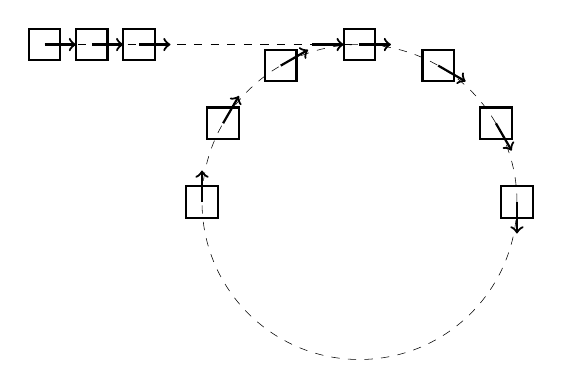
\begin{tikzpicture}[scale=2]
  % trace
  \draw[dashed, very thin] (-2cm, 1cm) -- (0, 1cm);
  \draw[dashed, very thin] (0,0) circle [radius=1cm];

  % leading nodes
  \foreach \x in {-2, -1.7, ..., -1.4} {
    \draw[thick] (\x cm, 1cm) +(-0.1, -0.1) rectangle ++(0.1, 0.1);
    \draw[thick, ->] (\x cm, 1cm) -- +(0.2, 0);
  }

  % cricular starting points
  \draw[thick, ->] (-0.3cm, 1cm) -- (-0.1cm, 1cm);

  % circular nodes
  \foreach \deg/\rot in {90/0, 60/-30, 30/-60, 0/-90, 180/90, 150/60, 120/30} {
    \draw[thick] (\deg : 1cm) +(-0.1, -0.1) rectangle ++(0.1, 0.1);
    \draw[thick, ->] (\deg : 1cm) -- +(\rot : 0.2);
  }
\end{tikzpicture}
\captionof{figure}{带有循环的列表}
\label{fig:circular-list}
\end{center}
}
\end{Exercise}

\begin{Answer}[ref = {ex:list-others}]
\Question{设计iota算法(希腊字母$I$)其用法如下:
  \begin{itemize}
  \item $iota(..., n) = [1, 2, 3, ..., n]$;
  \item $iota(m, n) = [m, m + 1, m + 2, ..., n]$,其中 $m \leq n$;
  \item $iota(m, m+a, ..., n) = [m, m + a, m + 2a, ..., m + ka]$; $k$是使得$m + ka \leq n$的最大整数。
  \item $iota(m, m, ...) = repeat(m) = [m, m, m, ...]$;
  \item $iota(m, ...) = [m, m + 1, m + 2, ... ]$.
  \end{itemize}

首先是尾递归的$[1, 2, ..., n]$:
\begin{Haskell}
iota = iota' [] where
  iota' ns n | n < 1 = ns
             | otherwise = iota' (n : ns) (n - 1)
\end{Haskell}

其次规定起始值:$[m, m + 1, ..., n]$,我们只需要把下限从1改为$m$即可:
\begin{Haskell}
iota m n = iota' [] n where
  iota' ns n | n < m = ns
             | otherwise = iota' (n : ns) (n - 1)
\end{Haskell}

其次规定步长:$[m, m + a, m + 2a, ..., m + ka]$,其中$k$是使$m + ka \leq n$的最大整数。

\begin{Haskell}
iota m n a | m <= n = m : iota (m + a) n a
           | otherwise = []
\end{Haskell}

为了产生$n = \infty$的开放序列:$[m, m + 1, ...]$,可以去掉上面的递归终止条件:
\begin{Haskell}
iota m = m : iota (m + 1)
\end{Haskell}

例如\texttt{take 10 (iota 1)}产生前10个自然数

把$+1$去掉就可以得到$repeat$
\begin{Haskell}
repeat m = m : repeat m
\end{Haskell}

综上,我们可以定义一个$iterate$函数,包含全部$iota$功能:
\begin{Haskell}
iterate f x = x : iterate f (f x)

iota1 n = take n $ iterate (+1) 1
iota2 m n = takeWhile (<=n) $ iterate (+1) m
iota3 m n a = takeWhile (<=n) $ iterate (+a) m
repeat m = iterate id m
iota5 m = iterate (+1) m
\end{Haskell}
}
\Question{实现线性时间的命令式$zip$算法。
\begin{Bourbaki}
[(A, B)] zip([A] xs, [B] ys) {
    [(A, B)] zs = null
    while xs != null and ys != null {
        zs = cons((xs.key, ys.key), zs)
        xs = xs.next
        ys = ys.next
    }
    return reverse(zs)
}
\end{Bourbaki}
}

\Question{用叠加定义$zip$(提示:定义两个列表的叠加$foldr2\ f\ z\ xs\ ys$)。

我们需要定义针对两个列表的叠加操作:

\be
\begin{array}{rcl}
foldr2\ f\ z\ [\ ]\ ys & = & z \\
foldr2\ f\ z\ xs\ [\ ] & = & z \\
foldr2\ f\ z\ (x \cons xs)\ (y \cons ys) & = & foldr2\ f\ (f\ x\ y\ z)\ xs\ ys \\
\end{array}
\ee

然后用$foldr2$定义$zip$(柯里化):

\[
zip = foldr2\ f\ [\ ], \text{其中}: f\ x\ y\ xys = (x, y) \cons xys
\]
}

\Question{使用$zip$实现$lastAt$。

为了实现右侧索引第$k$个元素,我们将$xs = [x_0, x_1, ..., x_{n-1}]$去掉前$k$个元素后得到$ys = drop\ k\ xs$。然后把$xs$、$ys$关联起来$zip\ xs\ ys$,这样最后一对元素就是$(x_{n-k-1}, x_{n-1})$。
\[
lastAt\ k\ xs = (fst \circ last)\ (zip\ xs\ (drop\ k\ xs))
\]
}

\Question{编写一个程序从列表中去除重复的元素。在命令式环境中,请用就地修改的方式删除这些重复元素。在纯函数环境中,构建一个只含有不同元素的新列表。结果列表中的元素顺序应保持和原列表中的一致。这一算法的复杂度是怎样的?如果允许使用额外的数据结构,可以如何简化实现?

\begin{Haskell}
dedup [] = []
dedup (x : xs) = x : dedup (filter (x /=) xs)
\end{Haskell}

可以用叠加来定义$dedup$:

\begin{Haskell}
dedup  = foldr f [] where
  f x xs = x : filter (x /=) xs
\end{Haskell}

由于对每个元素进行$filter$,复杂度为$O(n^2)$。使集合(见第三、四章)可以实现$O(n \lg n)$的去重操作:

\begin{Haskell}
dedup = Set.toList . Set.fromList
\end{Haskell}

对应的命令式就地修改实现为:
\begin{Bourbaki}
[K] dedup([K] xs) {
    Int n = length(xs)
    for Int i = 0, i < n, i++ {
        Int j = i + 1
        while j < n {
            if xs[i] == xs[j] {
                swap(xs[j], xs[n - 1])
                n--
            } else {
                j++
            }
        }
    }
    Int m = length(xs) - n
    loop m { pop(xs) }
    return xs
}
\end{Bourbaki}
}

\Question{可以用列表来表示十进制的非负整数。例如1024可以表示为:“$4 \rightarrow 2 \rightarrow 0 \rightarrow 1$”。一般来说,$n = d_m...d_2d_1$可以表示为:“$d_1 \rightarrow d_2 \rightarrow ... \rightarrow d_m$”。任给两个用列表表示的数$a$和$b$。实现它们的算数运算(加减乘除)。

\vspace{3mm}

把一个十进制自然数的各位上的数字放入列表,个位在左,高位在右。$n = (d_m...d_2d_1)_{10}$表示为[$d_1$, $d_2$, ..., $d_m$]。例如1024表示为[4, 2, 0, 1]。我们可以从这样的列表,通过$foldr\ (c\ d \mapsto 10d + c)\ 0$转换回自然数。反之,可以利用下面的函数将任意自然数转换成列表:

\begin{Haskell}
toList n | n < 10 = [n]
         | otherwise = (n `mod` 10) : toList (n `div` 10)
\end{Haskell}

首先实现加法。0是加法的单位元,即$0 + as = as + 0 = as$,其中$0$可以表示为$[\ ]$或$[0]$,所以:

\[
\begin{array}{rcl}
\left[ \ \right] + bs & = & bs \\
\left[ 0 \right] + bs & = & bs \\
as + \left[\ \right] & = & as \\
as + \left[ 0 \right] & = & as \\
\end{array}
\]

将各位相加$d = (a + b) \bmod 10$,进位为$c = \lfloor \dfrac{a + b}{10} \rfloor$,加到后续位上:

\[
(a \cons as) + (b \cons bs) = d \cons (as + bs + [c])
\]

下面是对应的例子程序:
\begin{Haskell}
add [] bs = bs
add as [] = as
add as [0] = as
add (a:as) (b:bs) = ((a + b) `mod` 10) : add as (add bs [(a + b) `div` 10])
\end{Haskell}

其次实现减法。$as - 0 = as$,表示为$as - [\ ] = as$。如果某一位上$a < b$,则需要借位:$d = 10 + a - b$,而剩余位$as' = as - [1]$。

\begin{Haskell}
minus as [] = as
minus (a:as) (b:bs) | a < b = (10 + a - b) : minus (minus as [1]) bs
                    | otherwise = (a - b) : minus as bs
\end{Haskell}

接下来实现乘法$as \times bs$,我们将$bs$中的每一位$b$乘以$as$,将结果乘以10后累加起来$cs' = 10 \times cs + (b \times as)$。计算$b \times as$时,如果$b = 0, 1$,结果为$0 \times as = 0$,$1 \times as = as$,其它情况下,用$b$乘以首位$a$得到$d = ab \bmod 10$,进位$c = \lfloor \dfrac{ab}{10} \rfloor$加到后继位乘法的结果上:

\[
b \times (a \cons as) = d : ([c] + (b \times as))
\]

对应的例子程序为:

\begin{Haskell}
mul as = foldr (\ b cs -> add (mul1 b as) (0:cs)) [] where
  mul1 0 _ = []
  mul1 1 as = as
  mul1 n [] = []
  mul1 n (a:as) = (n * a `mod` 10) : add [n * a `div` 10] (mul1 n as)
\end{Haskell}
}

%% \Question{给定一个0到10亿以内的数,编程将其转换为英文表示,例如123转换为“one hundred and twenty three”,如果带有小数部分呢?}

\Question{在命令式环境中,循环列表是一种有缺陷的列表:某个节点指向了以前的位置,如图\ref{fig:circular-list}所示。当遍历的时候,会陷入无限循环。设计一个算法检查某个列表是否含有循环。在此基础上,设计算法找到循环开始的节点(被两个不同祖先指向的节点)。
\begin{center}
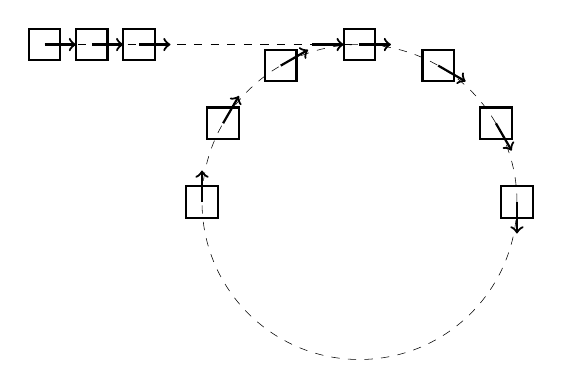
\begin{tikzpicture}[scale=2]
  % trace
  \draw[dashed, very thin] (-2cm, 1cm) -- (0, 1cm);
  \draw[dashed, very thin] (0,0) circle [radius=1cm];

  % leading nodes
  \foreach \x in {-2, -1.7, ..., -1.4} {
    \draw[thick] (\x cm, 1cm) +(-0.1, -0.1) rectangle ++(0.1, 0.1);
    \draw[thick, ->] (\x cm, 1cm) -- +(0.2, 0);
  }

  % cricular starting points
  \draw[thick, ->] (-0.3cm, 1cm) -- (-0.1cm, 1cm);

  % circular nodes
  \foreach \deg/\rot in {90/0, 60/-30, 30/-60, 0/-90, 180/90, 150/60, 120/30} {
    \draw[thick] (\deg : 1cm) +(-0.1, -0.1) rectangle ++(0.1, 0.1);
    \draw[thick, ->] (\deg : 1cm) -- +(\rot : 0.2);
  }
\end{tikzpicture}
\captionof{figure}{带有循环的列表}
\label{fig:circular-list}
\end{center}
}
\end{Answer}

\ifx\wholebook\relax \else
\section{参考答案}
\shipoutAnswer

\begin{thebibliography}{99}

\bibitem{fp-pearls}
Richard Bird. ``Pearls of Functional Algorithm Design''. Cambridge University Press; 1 edition (November 1, 2010). ISBN: 978-0521513388

\bibitem{slpj-book-1987}
Simon L. Peyton Jones. ``The Implementation of Functional Programming Languages''. Prentice-Hall International Series in Computer Since. Prentice Hall (May 1987). ISBN: 978-0134533339

\bibitem{moderncxx}
Andrei Alexandrescu. ``Modern C++ design: Generic Programming and Design Patterns Applied''. Addison Wesley February 01, 2001, ISBN 0-201-70431-5

\bibitem{mittype}
Benjamin C. Pierce. ``Types and Programming Languages''. The MIT Press, 2002. ISBN:0262162091

\bibitem{unplugged}
刘新宇. ``同构——编程中的数学''. 2020. \url{https://github.com/liuxinyu95/unplugged}

\bibitem{SICP}
Harold Abelson, Gerald Jay Sussman, Julie Sussman. ``Structure and Interpretation of Computer Programs, 2nd Edition''. MIT Press, 1996, ISBN 0-262-51087-1

\bibitem{okasaki-book}
Chris Okasaki. ``Purely Functional Data Structures''. Cambridge university press, (July 1, 1999), ISBN-13: 978-0521663502

\bibitem{algo-fp}
Fethi Rabhi, Guy Lapalme. ``Algorithms: a functional programming approach''. Second edition. Addison-Wesley, 1999. ISBN: 0201-59604-0

\bibitem{learn-haskell}
Miran Lipovaca. ``Learn You a Haskell for Great Good! A Beginner's Guide''. No Starch Press; 1 edition April 2011, 400 pp. ISBN: 978-1-59327-283-8

\bibitem{erlang}
Joe Armstrong. ``Programming Erlang: Software for a Concurrent World''. Pragmatic Bookshelf; 1 edition (July 18, 2007). ISBN-13: 978-1934356005

\bibitem{wiki-tail-call}
Wikipedia. ``Tail call''. \url{https://en.wikipedia.org/wiki/Tail_call}

\bibitem{sgi-stl-transform}
SGI. ``transform''. \url{http://www.sgi.com/tech/stl/transform.html}

\bibitem{poj-drunk-jailer}
ACM/ICPC. ``The drunk jailer.'' Peking University judge online for ACM/ICPC. \url{http://poj.org/problem?id=1218}.

\bibitem{Haskell-wiki}
Haskell wiki. ``Haskell programming tips''. 4.4 Choose the appropriate fold. \url{http://www.haskell.org/haskellwiki/Haskell_programming_tips}

\bibitem{wiki-dot-product}
Wikipedia. ``Dot product''. \url{https://en.wikipedia.org/wiki/Dot_product}

\end{thebibliography}

\expandafter\enddocument
\fi
